% Options for packages loaded elsewhere
\PassOptionsToPackage{unicode}{hyperref}
\PassOptionsToPackage{hyphens}{url}
%
\documentclass[
  11pt,
]{article}
\usepackage{amsmath,amssymb}
\usepackage{iftex}
\ifPDFTeX
  \usepackage[T1]{fontenc}
  \usepackage[utf8]{inputenc}
  \usepackage{textcomp} % provide euro and other symbols
\else % if luatex or xetex
  \usepackage{unicode-math} % this also loads fontspec
  \defaultfontfeatures{Scale=MatchLowercase}
  \defaultfontfeatures[\rmfamily]{Ligatures=TeX,Scale=1}
\fi
\usepackage{lmodern}
\ifPDFTeX\else
  % xetex/luatex font selection
\fi
% Use upquote if available, for straight quotes in verbatim environments
\IfFileExists{upquote.sty}{\usepackage{upquote}}{}
\IfFileExists{microtype.sty}{% use microtype if available
  \usepackage[]{microtype}
  \UseMicrotypeSet[protrusion]{basicmath} % disable protrusion for tt fonts
}{}
\makeatletter
\@ifundefined{KOMAClassName}{% if non-KOMA class
  \IfFileExists{parskip.sty}{%
    \usepackage{parskip}
  }{% else
    \setlength{\parindent}{0pt}
    \setlength{\parskip}{6pt plus 2pt minus 1pt}}
}{% if KOMA class
  \KOMAoptions{parskip=half}}
\makeatother
\usepackage{xcolor}
\usepackage[margin = 0.5in]{geometry}
\usepackage{color}
\usepackage{fancyvrb}
\newcommand{\VerbBar}{|}
\newcommand{\VERB}{\Verb[commandchars=\\\{\}]}
\DefineVerbatimEnvironment{Highlighting}{Verbatim}{commandchars=\\\{\}}
% Add ',fontsize=\small' for more characters per line
\usepackage{framed}
\definecolor{shadecolor}{RGB}{248,248,248}
\newenvironment{Shaded}{\begin{snugshade}}{\end{snugshade}}
\newcommand{\AlertTok}[1]{\textcolor[rgb]{0.94,0.16,0.16}{#1}}
\newcommand{\AnnotationTok}[1]{\textcolor[rgb]{0.56,0.35,0.01}{\textbf{\textit{#1}}}}
\newcommand{\AttributeTok}[1]{\textcolor[rgb]{0.13,0.29,0.53}{#1}}
\newcommand{\BaseNTok}[1]{\textcolor[rgb]{0.00,0.00,0.81}{#1}}
\newcommand{\BuiltInTok}[1]{#1}
\newcommand{\CharTok}[1]{\textcolor[rgb]{0.31,0.60,0.02}{#1}}
\newcommand{\CommentTok}[1]{\textcolor[rgb]{0.56,0.35,0.01}{\textit{#1}}}
\newcommand{\CommentVarTok}[1]{\textcolor[rgb]{0.56,0.35,0.01}{\textbf{\textit{#1}}}}
\newcommand{\ConstantTok}[1]{\textcolor[rgb]{0.56,0.35,0.01}{#1}}
\newcommand{\ControlFlowTok}[1]{\textcolor[rgb]{0.13,0.29,0.53}{\textbf{#1}}}
\newcommand{\DataTypeTok}[1]{\textcolor[rgb]{0.13,0.29,0.53}{#1}}
\newcommand{\DecValTok}[1]{\textcolor[rgb]{0.00,0.00,0.81}{#1}}
\newcommand{\DocumentationTok}[1]{\textcolor[rgb]{0.56,0.35,0.01}{\textbf{\textit{#1}}}}
\newcommand{\ErrorTok}[1]{\textcolor[rgb]{0.64,0.00,0.00}{\textbf{#1}}}
\newcommand{\ExtensionTok}[1]{#1}
\newcommand{\FloatTok}[1]{\textcolor[rgb]{0.00,0.00,0.81}{#1}}
\newcommand{\FunctionTok}[1]{\textcolor[rgb]{0.13,0.29,0.53}{\textbf{#1}}}
\newcommand{\ImportTok}[1]{#1}
\newcommand{\InformationTok}[1]{\textcolor[rgb]{0.56,0.35,0.01}{\textbf{\textit{#1}}}}
\newcommand{\KeywordTok}[1]{\textcolor[rgb]{0.13,0.29,0.53}{\textbf{#1}}}
\newcommand{\NormalTok}[1]{#1}
\newcommand{\OperatorTok}[1]{\textcolor[rgb]{0.81,0.36,0.00}{\textbf{#1}}}
\newcommand{\OtherTok}[1]{\textcolor[rgb]{0.56,0.35,0.01}{#1}}
\newcommand{\PreprocessorTok}[1]{\textcolor[rgb]{0.56,0.35,0.01}{\textit{#1}}}
\newcommand{\RegionMarkerTok}[1]{#1}
\newcommand{\SpecialCharTok}[1]{\textcolor[rgb]{0.81,0.36,0.00}{\textbf{#1}}}
\newcommand{\SpecialStringTok}[1]{\textcolor[rgb]{0.31,0.60,0.02}{#1}}
\newcommand{\StringTok}[1]{\textcolor[rgb]{0.31,0.60,0.02}{#1}}
\newcommand{\VariableTok}[1]{\textcolor[rgb]{0.00,0.00,0.00}{#1}}
\newcommand{\VerbatimStringTok}[1]{\textcolor[rgb]{0.31,0.60,0.02}{#1}}
\newcommand{\WarningTok}[1]{\textcolor[rgb]{0.56,0.35,0.01}{\textbf{\textit{#1}}}}
\usepackage{longtable,booktabs,array}
\usepackage{calc} % for calculating minipage widths
% Correct order of tables after \paragraph or \subparagraph
\usepackage{etoolbox}
\makeatletter
\patchcmd\longtable{\par}{\if@noskipsec\mbox{}\fi\par}{}{}
\makeatother
% Allow footnotes in longtable head/foot
\IfFileExists{footnotehyper.sty}{\usepackage{footnotehyper}}{\usepackage{footnote}}
\makesavenoteenv{longtable}
\usepackage{graphicx}
\makeatletter
\def\maxwidth{\ifdim\Gin@nat@width>\linewidth\linewidth\else\Gin@nat@width\fi}
\def\maxheight{\ifdim\Gin@nat@height>\textheight\textheight\else\Gin@nat@height\fi}
\makeatother
% Scale images if necessary, so that they will not overflow the page
% margins by default, and it is still possible to overwrite the defaults
% using explicit options in \includegraphics[width, height, ...]{}
\setkeys{Gin}{width=\maxwidth,height=\maxheight,keepaspectratio}
% Set default figure placement to htbp
\makeatletter
\def\fps@figure{htbp}
\makeatother
\setlength{\emergencystretch}{3em} % prevent overfull lines
\providecommand{\tightlist}{%
  \setlength{\itemsep}{0pt}\setlength{\parskip}{0pt}}
\setcounter{secnumdepth}{5}
\usepackage{amsmath}
\usepackage{amssymb}
\usepackage{amsfonts}
\usepackage{amsthm}
\usepackage{fancyhdr}
\pagestyle{fancy}
\fancyhf{}
\rhead{Owusu Noah}
\lhead{GAM, MARS, and PPR}
\cfoot{\thepage}
\usepackage{algorithm}
\usepackage[noend]{algpseudocode}
\usepackage{booktabs}
\usepackage{longtable}
\usepackage{array}
\usepackage{multirow}
\usepackage{wrapfig}
\usepackage{float}
\usepackage{colortbl}
\usepackage{pdflscape}
\usepackage{tabu}
\usepackage{threeparttable}
\usepackage{threeparttablex}
\usepackage[normalem]{ulem}
\usepackage{makecell}
\usepackage{xcolor}
\ifLuaTeX
  \usepackage{selnolig}  % disable illegal ligatures
\fi
\IfFileExists{bookmark.sty}{\usepackage{bookmark}}{\usepackage{hyperref}}
\IfFileExists{xurl.sty}{\usepackage{xurl}}{} % add URL line breaks if available
\urlstyle{same}
\hypersetup{
  pdftitle={Project VI: GAM, MARS, and PPR},
  pdfauthor={Owusu Noah},
  hidelinks,
  pdfcreator={LaTeX via pandoc}}

\title{Project VI: GAM, MARS, and PPR}
\author{Owusu Noah}
\date{09 26, 2023}

\begin{document}
\maketitle

{
\setcounter{tocdepth}{4}
\tableofcontents
}
\newpage
\section{Question 1 - Data Preparation}

\subsection{Importing the data}

\begin{Shaded}
\begin{Highlighting}[]
\FunctionTok{library}\NormalTok{(dplyr)}
\NormalTok{hr }\OtherTok{\textless{}{-}} \StringTok{"HR\_comma\_sep.csv"} \SpecialCharTok{\%\textgreater{}\%} 
  \FunctionTok{read.csv}\NormalTok{()}

\FunctionTok{head}\NormalTok{(hr); }\FunctionTok{dim}\NormalTok{(hr)}
\end{Highlighting}
\end{Shaded}

\begin{verbatim}
##   satisfaction_level last_evaluation number_project average_montly_hours
## 1               0.38            0.53              2                  157
## 2               0.80            0.86              5                  262
## 3               0.11            0.88              7                  272
## 4               0.72            0.87              5                  223
## 5               0.37            0.52              2                  159
## 6               0.41            0.50              2                  153
##   time_spend_company Work_accident left promotion_last_5years sales salary
## 1                  3             0    1                     0 sales    low
## 2                  6             0    1                     0 sales medium
## 3                  4             0    1                     0 sales medium
## 4                  5             0    1                     0 sales    low
## 5                  3             0    1                     0 sales    low
## 6                  3             0    1                     0 sales    low
\end{verbatim}

\begin{verbatim}
## [1] 14999    10
\end{verbatim}

\textbf{Comment:}

The \textbf{HR} data has \(14999\) observations and \(10\) variables,
namely \textbf{satisfaction\_level} ,\textbf{number of project} etc.

\subsubsection{Changing the categorical variable \textit{salary} to ordinal}

\begin{Shaded}
\begin{Highlighting}[]
\NormalTok{hr}\SpecialCharTok{$}\NormalTok{salary }\OtherTok{\textless{}{-}} \FunctionTok{factor}\NormalTok{(hr}\SpecialCharTok{$}\NormalTok{salary, }
        \AttributeTok{levels=}\FunctionTok{c}\NormalTok{(}\StringTok{"low"}\NormalTok{, }\StringTok{"medium"}\NormalTok{,}\StringTok{"high"}\NormalTok{), }\AttributeTok{ordered=}\ConstantTok{TRUE}\NormalTok{)}

\FunctionTok{class}\NormalTok{(hr}\SpecialCharTok{$}\NormalTok{salary)}
\end{Highlighting}
\end{Shaded}

\begin{verbatim}
## [1] "ordered" "factor"
\end{verbatim}

\newpage
\subsubsection{Changing the column name of variable sales to department}

\begin{Shaded}
\begin{Highlighting}[]
\FunctionTok{colnames}\NormalTok{(hr)[}\FunctionTok{colnames}\NormalTok{(hr) }\SpecialCharTok{==} \StringTok{\textquotesingle{}sales\textquotesingle{}}\NormalTok{] }\OtherTok{\textless{}{-}} \StringTok{\textquotesingle{}department\textquotesingle{}}
  
\FunctionTok{head}\NormalTok{(hr, }\DecValTok{2}\NormalTok{)}
\end{Highlighting}
\end{Shaded}

\begin{verbatim}
##   satisfaction_level last_evaluation number_project average_montly_hours
## 1               0.38            0.53              2                  157
## 2               0.80            0.86              5                  262
##   time_spend_company Work_accident left promotion_last_5years department salary
## 1                  3             0    1                     0      sales    low
## 2                  6             0    1                     0      sales medium
\end{verbatim}

\subsubsection{Converting the target variable "left" to categorical variable}

\begin{Shaded}
\begin{Highlighting}[]
\NormalTok{hr}\SpecialCharTok{$}\NormalTok{left }\OtherTok{\textless{}{-}} \FunctionTok{factor}\NormalTok{(hr}\SpecialCharTok{$}\NormalTok{left, }\AttributeTok{levels =} \FunctionTok{c}\NormalTok{(}\DecValTok{0}\NormalTok{,}\DecValTok{1}\NormalTok{), }\AttributeTok{labels =} \FunctionTok{c}\NormalTok{(}\StringTok{"stayed"}\NormalTok{, }\StringTok{"left"}\NormalTok{))}
\FunctionTok{class}\NormalTok{(hr}\SpecialCharTok{$}\NormalTok{left)}
\end{Highlighting}
\end{Shaded}

\begin{verbatim}
## [1] "factor"
\end{verbatim}

\textbf{Comment:}

Yes! the target variable \textbf{left} is now a categorical variable.

\subsubsection{Inspecting missing values}

\begin{Shaded}
\begin{Highlighting}[]
\CommentTok{\# Listing the missing rate for each variable.}
\NormalTok{miss.info }\OtherTok{\textless{}{-}} \ControlFlowTok{function}\NormalTok{(dat, }\AttributeTok{filename=}\ConstantTok{NULL}\NormalTok{)\{}
\NormalTok{  vnames }\OtherTok{\textless{}{-}} \FunctionTok{colnames}\NormalTok{(dat); vnames}
\NormalTok{  n }\OtherTok{\textless{}{-}} \FunctionTok{nrow}\NormalTok{(dat)}
\NormalTok{  out }\OtherTok{\textless{}{-}} \ConstantTok{NULL}
  \ControlFlowTok{for}\NormalTok{ (j }\ControlFlowTok{in} \DecValTok{1}\SpecialCharTok{:} \FunctionTok{ncol}\NormalTok{(dat))\{}
\NormalTok{    vname }\OtherTok{\textless{}{-}} \FunctionTok{colnames}\NormalTok{(dat)[j]}
\NormalTok{    x }\OtherTok{\textless{}{-}} \FunctionTok{as.vector}\NormalTok{(dat[,j])}
\NormalTok{    n1 }\OtherTok{\textless{}{-}} \FunctionTok{sum}\NormalTok{(}\FunctionTok{is.na}\NormalTok{(x), }\AttributeTok{na.rm=}\NormalTok{T)}
\NormalTok{    n2 }\OtherTok{\textless{}{-}} \FunctionTok{sum}\NormalTok{(x}\SpecialCharTok{==}\StringTok{"NA"}\NormalTok{, }\AttributeTok{na.rm=}\NormalTok{T)}
\NormalTok{    n3 }\OtherTok{\textless{}{-}} \FunctionTok{sum}\NormalTok{(x}\SpecialCharTok{==}\StringTok{""}\NormalTok{, }\AttributeTok{na.rm=}\NormalTok{T)}
\NormalTok{    nmiss }\OtherTok{\textless{}{-}}\NormalTok{ n1 }\SpecialCharTok{+}\NormalTok{ n2 }\SpecialCharTok{+}\NormalTok{ n3}
\NormalTok{    ncomplete }\OtherTok{\textless{}{-}}\NormalTok{ n}\SpecialCharTok{{-}}\NormalTok{nmiss}
\NormalTok{    out }\OtherTok{\textless{}{-}} \FunctionTok{rbind}\NormalTok{(out, }\FunctionTok{c}\NormalTok{(}\AttributeTok{col.number=}\NormalTok{j, }\AttributeTok{vname=}\NormalTok{vname, }
                        \AttributeTok{mode=}\FunctionTok{mode}\NormalTok{(x), }\AttributeTok{n.levels=}\FunctionTok{length}\NormalTok{(}\FunctionTok{unique}\NormalTok{(x)), }
                        \AttributeTok{ncomplete=}\NormalTok{ncomplete, }\AttributeTok{miss.perc=}\NormalTok{nmiss}\SpecialCharTok{/}\NormalTok{n))}
\NormalTok{  \}}
\NormalTok{  out }\OtherTok{\textless{}{-}} \FunctionTok{as.data.frame}\NormalTok{(out)}
  \FunctionTok{row.names}\NormalTok{(out) }\OtherTok{\textless{}{-}} \ConstantTok{NULL} 
  \ControlFlowTok{if}\NormalTok{ (}\SpecialCharTok{!}\FunctionTok{is.null}\NormalTok{(filename)) }\FunctionTok{write.csv}\NormalTok{(out, }\AttributeTok{file =}\NormalTok{ filename, }\AttributeTok{row.names=}\NormalTok{F)}
  \FunctionTok{return}\NormalTok{(out)}
\NormalTok{\}}
\NormalTok{df }\OtherTok{\textless{}{-}}\NormalTok{ knitr}\SpecialCharTok{::}\FunctionTok{kable}\NormalTok{(}\FunctionTok{miss.info}\NormalTok{(hr), }\AttributeTok{booktabs =}\NormalTok{ T, }\AttributeTok{format =} \StringTok{"markdown"}\NormalTok{) }
\NormalTok{kableExtra}\SpecialCharTok{::}\FunctionTok{kable\_styling}\NormalTok{(df, }\AttributeTok{bootstrap\_options =} \StringTok{"striped"}\NormalTok{, }\AttributeTok{full\_width =}\NormalTok{ F)}
\end{Highlighting}
\end{Shaded}

\begin{longtable}[]{@{}
  >{\raggedright\arraybackslash}p{(\columnwidth - 10\tabcolsep) * \real{0.1528}}
  >{\raggedright\arraybackslash}p{(\columnwidth - 10\tabcolsep) * \real{0.3056}}
  >{\raggedright\arraybackslash}p{(\columnwidth - 10\tabcolsep) * \real{0.1389}}
  >{\raggedright\arraybackslash}p{(\columnwidth - 10\tabcolsep) * \real{0.1250}}
  >{\raggedright\arraybackslash}p{(\columnwidth - 10\tabcolsep) * \real{0.1389}}
  >{\raggedright\arraybackslash}p{(\columnwidth - 10\tabcolsep) * \real{0.1389}}@{}}
\toprule\noalign{}
\begin{minipage}[b]{\linewidth}\raggedright
col.number
\end{minipage} & \begin{minipage}[b]{\linewidth}\raggedright
vname
\end{minipage} & \begin{minipage}[b]{\linewidth}\raggedright
mode
\end{minipage} & \begin{minipage}[b]{\linewidth}\raggedright
n.levels
\end{minipage} & \begin{minipage}[b]{\linewidth}\raggedright
ncomplete
\end{minipage} & \begin{minipage}[b]{\linewidth}\raggedright
miss.perc
\end{minipage} \\
\midrule\noalign{}
\endhead
\bottomrule\noalign{}
\endlastfoot
1 & satisfaction\_level & numeric & 92 & 14999 & 0 \\
2 & last\_evaluation & numeric & 65 & 14999 & 0 \\
3 & number\_project & numeric & 6 & 14999 & 0 \\
4 & average\_montly\_hours & numeric & 215 & 14999 & 0 \\
5 & time\_spend\_company & numeric & 8 & 14999 & 0 \\
6 & Work\_accident & numeric & 2 & 14999 & 0 \\
7 & left & character & 2 & 14999 & 0 \\
8 & promotion\_last\_5years & numeric & 2 & 14999 & 0 \\
9 & department & character & 10 & 14999 & 0 \\
10 & salary & character & 3 & 14999 & 0 \\
\end{longtable}

\textbf{Comment:}

From the above table, it is clear that the \textbf{hr} dataset have no
missing value.This is a desired outcome to guarantee a reliable
conclusion and practicable subsequent analysis.

\newpage
\section{Question 2 - Exploratory Data Analysis}

\subsection{Checking for variable type}

\begin{Shaded}
\begin{Highlighting}[]
\FunctionTok{glimpse}\NormalTok{(hr)}
\end{Highlighting}
\end{Shaded}

\begin{verbatim}
## Rows: 14,999
## Columns: 10
## $ satisfaction_level    <dbl> 0.38, 0.80, 0.11, 0.72, 0.37, 0.41, 0.10, 0.92, ~
## $ last_evaluation       <dbl> 0.53, 0.86, 0.88, 0.87, 0.52, 0.50, 0.77, 0.85, ~
## $ number_project        <int> 2, 5, 7, 5, 2, 2, 6, 5, 5, 2, 2, 6, 4, 2, 2, 2, ~
## $ average_montly_hours  <int> 157, 262, 272, 223, 159, 153, 247, 259, 224, 142~
## $ time_spend_company    <int> 3, 6, 4, 5, 3, 3, 4, 5, 5, 3, 3, 4, 5, 3, 3, 3, ~
## $ Work_accident         <int> 0, 0, 0, 0, 0, 0, 0, 0, 0, 0, 0, 0, 0, 0, 0, 0, ~
## $ left                  <fct> left, left, left, left, left, left, left, left, ~
## $ promotion_last_5years <int> 0, 0, 0, 0, 0, 0, 0, 0, 0, 0, 0, 0, 0, 0, 0, 0, ~
## $ department            <chr> "sales", "sales", "sales", "sales", "sales", "sa~
## $ salary                <ord> low, medium, medium, low, low, low, low, low, lo~
\end{verbatim}

\textbf{Comment:}

From the above output, variables \textbf{satisfaction\_level} and
\textbf{last\_evaluation} are numeric(continuous) variable,
\textbf{salary} is categorical (ordinal) variable , and \textbf{sales
and left} are categorical (nominal) variable. The remaining variables
are numeric(integer) variable.

\subsection{Frequency distribution of target variable}

\begin{Shaded}
\begin{Highlighting}[]
\CommentTok{\#Inspecting frequency distribution of the target variable (left)}
\FunctionTok{tab1}\NormalTok{(hr}\SpecialCharTok{$}\NormalTok{left, }\AttributeTok{decimal =} \DecValTok{2}\NormalTok{, }\AttributeTok{cum.percent =}\NormalTok{ F, }\AttributeTok{xlab =} \StringTok{"Left the company"}\NormalTok{, }\AttributeTok{ylab =} \StringTok{"Frequency"}\NormalTok{, }\AttributeTok{col =} \StringTok{"blue"}\NormalTok{)}
\end{Highlighting}
\end{Shaded}

\includegraphics[width=0.9\linewidth]{OWUSU_project_files/figure-latex/unnamed-chunk-7-1}

\begin{verbatim}
## hr$left : 
##         Frequency Percent
## stayed      11428   76.19
## left         3571   23.81
##   Total     14999  100.00
\end{verbatim}

\text{Comment:}

The frequency table revealed 11428(76.19\%) \textbf{stayed} counts and
3571(23.81\%) \textbf{left} counts for the \textbf{left} variable. This
classification case is neither completely balanced nor unbalanced.
However, we will consider this scenario as a balanced classification and
continue with our analysis since the proportion of employees who left is
greater than 5\% (which is the cutoff proportion for imbalanced
classification).

\hfill\break
\textbf{(2a)}

\subsection{Scatterplot of employees Satisfaction level vrs Number of project}

\begin{Shaded}
\begin{Highlighting}[]
\FunctionTok{ggplot}\NormalTok{(}\AttributeTok{data =}\NormalTok{ hr, }\FunctionTok{aes}\NormalTok{(}\AttributeTok{x=}\NormalTok{ number\_project, }\AttributeTok{color =}\NormalTok{ left))}\SpecialCharTok{+}
  \FunctionTok{geom\_point}\NormalTok{(}\AttributeTok{position=}\FunctionTok{position\_jitterdodge}\NormalTok{(),}\AttributeTok{alpha=}\NormalTok{.}\DecValTok{5}\NormalTok{,}
             \FunctionTok{aes}\NormalTok{ (}\AttributeTok{y =}\NormalTok{   satisfaction\_level), }\AttributeTok{bins =} \DecValTok{2}\NormalTok{) }\SpecialCharTok{+}
  \FunctionTok{scale\_color\_manual}\NormalTok{(}\StringTok{"Status"}\NormalTok{, }\AttributeTok{values =} \FunctionTok{c}\NormalTok{(}\StringTok{"cyan2"}\NormalTok{, }\StringTok{"orange"}\NormalTok{))}
\end{Highlighting}
\end{Shaded}

\includegraphics[width=0.9\linewidth]{OWUSU_project_files/figure-latex/unnamed-chunk-8-1}

\begin{Shaded}
\begin{Highlighting}[]
   \FunctionTok{labs}\NormalTok{(}\AttributeTok{title =} 
\StringTok{"Employee\textquotesingle{}s Satisfaction level vrs Number of projects (Left the Comapny {-} stayed/left)"}\NormalTok{,}
           \AttributeTok{x =} \StringTok{"Number of projects"}\NormalTok{, }\AttributeTok{y =} \StringTok{"Satisfaction level"}\NormalTok{)}\SpecialCharTok{+}
            \FunctionTok{theme}\NormalTok{(}\AttributeTok{plot.title =} \FunctionTok{element\_text}\NormalTok{(}\AttributeTok{size=}\DecValTok{9}\NormalTok{),}
                   \AttributeTok{axis.text.x =} \FunctionTok{element\_text}\NormalTok{(}\AttributeTok{size=}\DecValTok{6}\NormalTok{) )}
\end{Highlighting}
\end{Shaded}

\begin{verbatim}
## NULL
\end{verbatim}

\hfill\break

\textbf{Comment:}

From the plot above, we can see that employees who are satisfied with
their work are less willing to leave. Thus, the more satisfied employees
are, the less willingly they are to leave. However, the interesting
thing is that we can find that not all employees with low-paying and
unsatisfactory jobs left the company. Most of them continued working
with the company. Finding these employees and understanding why they are
unwilling to leave can provide valuable information to the HR
department. Moreover, Among employees who left, had \textbf{2
number\_project} were not satisfied since majority of them had
satisfaction level below \(0.50\)

\hfill\break
\textbf{(2b)}

\subsection{Correlation matrix among the variables in the \textbf{hr} dataset}

\begin{Shaded}
\begin{Highlighting}[]
\FunctionTok{library}\NormalTok{(GoodmanKruskal)}
\NormalTok{mat.hr }\OtherTok{\textless{}{-}} \FunctionTok{GKtauDataframe}\NormalTok{(hr)}
\FunctionTok{plot}\NormalTok{(mat.hr, }\AttributeTok{dgts =} \DecValTok{2}\NormalTok{, }\AttributeTok{diagSize =} \FloatTok{0.8}\NormalTok{)}
\end{Highlighting}
\end{Shaded}

\includegraphics[width=0.9\linewidth]{OWUSU_project_files/figure-latex/unnamed-chunk-9-1}

\hfill\break
\textbf{Comment:}

After carefully examining the data, The variables
\textbf{satisfaction\_level, last\_evaluation, number\_project} and
\textbf{average\_monthly\_hours} exhibit slight forward associations
with the target variable \textbf{left}, the reverse associations are
much smaller.

The variable \textbf{satisfaction\_level} exhibits a slight ability to
explain variations in the other variables (ranging from \textbf{0.01} to
\textbf{0.53}), the reverse associations are much smaller: the \(\tau\)
value from \textbf{satisfaction\_level} to \textbf{left} is
\textbf{0.53},indicating quite a strong association while that from
\textbf{satisfaction\_level} to \textbf{number\_project} is
\textbf{0.18}.

\subsection{Interesting finding 1}

\textbf{Salary VRS. Employee turnover}

\begin{Shaded}
\begin{Highlighting}[]
\NormalTok{t1 }\OtherTok{\textless{}{-}} \FunctionTok{table}\NormalTok{(hr}\SpecialCharTok{$}\NormalTok{salary,hr}\SpecialCharTok{$}\NormalTok{left)}
\NormalTok{df }\OtherTok{\textless{}{-}} \FunctionTok{as.data.frame}\NormalTok{(}\FunctionTok{prop.table}\NormalTok{(t1))}

\CommentTok{\#round(prop.table(t1), 3)}

\FunctionTok{ggplot}\NormalTok{(df, }\FunctionTok{aes}\NormalTok{(}\AttributeTok{x=}\NormalTok{Var1,}\AttributeTok{y=}\NormalTok{Freq,}\AttributeTok{fill=}\NormalTok{Var2)) }\SpecialCharTok{+}
  \FunctionTok{geom\_bar}\NormalTok{(}\AttributeTok{position=}\StringTok{"dodge"}\NormalTok{,}\AttributeTok{stat=}\StringTok{\textquotesingle{}identity\textquotesingle{}}\NormalTok{)}\SpecialCharTok{+}
  \FunctionTok{ggtitle}\NormalTok{(}\StringTok{"Barplot of salary vrs left"}\NormalTok{)}\SpecialCharTok{+}
  \FunctionTok{xlab}\NormalTok{(}\StringTok{"Salary category"}\NormalTok{)}\SpecialCharTok{+} \FunctionTok{ylab}\NormalTok{(}\StringTok{"Proportion of employess"}\NormalTok{)}\SpecialCharTok{+}
  \FunctionTok{scale\_fill\_manual}\NormalTok{(}\AttributeTok{values =} \FunctionTok{c}\NormalTok{(}\StringTok{"cyan2"}\NormalTok{,}\StringTok{"orange"}\NormalTok{))}
\end{Highlighting}
\end{Shaded}

\includegraphics[width=0.9\linewidth]{OWUSU_project_files/figure-latex/unnamed-chunk-10-1}

\hfill\break
\textbf{Comment:} From the above results, the data indicates that
employees who left the company tend to have lower salaries when compared
to employees who do not.

Among the employees who left the company, majority received low and
medium salaries.

\hfill\break

\subsection{Interesting finding 2}

The frequency distribution of time spent by employees in the company
were first explored and a graphical representation drawn after using a
barplot.

\begin{Shaded}
\begin{Highlighting}[]
\FunctionTok{table}\NormalTok{(hr}\SpecialCharTok{$}\NormalTok{time\_spend\_company)}
\end{Highlighting}
\end{Shaded}

\begin{verbatim}
## 
##    2    3    4    5    6    7    8   10 
## 3244 6443 2557 1473  718  188  162  214
\end{verbatim}

\begin{Shaded}
\begin{Highlighting}[]
\FunctionTok{ggplot}\NormalTok{(}\AttributeTok{data =}\NormalTok{ hr, }\FunctionTok{aes}\NormalTok{(}\AttributeTok{x =}\NormalTok{ time\_spend\_company, }\AttributeTok{y =}\NormalTok{ ..count..))}\SpecialCharTok{+} 
  \FunctionTok{geom\_bar}\NormalTok{(}\AttributeTok{fill =} \FunctionTok{c}\NormalTok{(}\DecValTok{3}\NormalTok{,}\DecValTok{5}\NormalTok{,}\DecValTok{7}\NormalTok{,}\DecValTok{9}\NormalTok{,}\DecValTok{11}\NormalTok{,}\DecValTok{13}\NormalTok{,}\DecValTok{15}\NormalTok{,}\DecValTok{6}\NormalTok{), }
                     \AttributeTok{alpha =} \FloatTok{0.6}\NormalTok{)}\SpecialCharTok{+}
  \FunctionTok{scale\_x\_continuous}\NormalTok{(}\AttributeTok{breaks=} \FunctionTok{seq}\NormalTok{(}\DecValTok{0}\NormalTok{,}\DecValTok{10}\NormalTok{,}\DecValTok{1}\NormalTok{))}\SpecialCharTok{+}
  \FunctionTok{theme\_bw}\NormalTok{()}\SpecialCharTok{+}
  \FunctionTok{ggtitle}\NormalTok{(}\StringTok{"Years in company"}\NormalTok{)}\SpecialCharTok{+}
  \FunctionTok{theme}\NormalTok{(}\AttributeTok{plot.title =} \FunctionTok{element\_text}\NormalTok{(}\AttributeTok{hjust =} \FloatTok{0.5}\NormalTok{))}\SpecialCharTok{+}
  \FunctionTok{labs}\NormalTok{(}\AttributeTok{x =} \StringTok{"Years"}\NormalTok{, }\AttributeTok{y =} \StringTok{"Number of employees"}\NormalTok{)}\SpecialCharTok{+}
  \FunctionTok{theme}\NormalTok{(}\AttributeTok{plot.title =} \FunctionTok{element\_text}\NormalTok{(}\AttributeTok{size =} \DecValTok{13}\NormalTok{,}\AttributeTok{face =} \StringTok{"bold"}\NormalTok{),}
              \AttributeTok{text =} \FunctionTok{element\_text}\NormalTok{(}\AttributeTok{size =} \DecValTok{10}\NormalTok{))}
\end{Highlighting}
\end{Shaded}

\includegraphics[width=0.9\linewidth]{OWUSU_project_files/figure-latex/unnamed-chunk-12-1}

\hfill\break
\textbf{Comment:}

The range of time spent by an employee in the company is \emph{2} to
\emph{10} years with \emph{no} employee working for \emph{9} years. It
can also be seen from the above figure that over 6000 employees in the
company spent \emph{three years} whilst a few employees spent
\emph{eight years} with the company.

\hfill\break

\subsection{Interesting finding 3}

\textbf{Distribution of features grouped by the target variable}

\begin{Shaded}
\begin{Highlighting}[]
\NormalTok{OverlayedHist }\OtherTok{\textless{}{-}} \ControlFlowTok{function}\NormalTok{(mData, featureVar, grouper, mbinwidth, mTitle,  mxlab,}
\NormalTok{                          mylab, mlegendTitle)\{}
  
\NormalTok{  p }\OtherTok{\textless{}{-}} \FunctionTok{ggplot}\NormalTok{(hr, }\FunctionTok{aes}\NormalTok{(}\FunctionTok{eval}\NormalTok{(}\FunctionTok{parse}\NormalTok{(}\AttributeTok{text =}\NormalTok{ featureVar)), }\AttributeTok{fill =} \FunctionTok{eval}\NormalTok{(}\FunctionTok{parse}\NormalTok{(}\AttributeTok{text =}\NormalTok{ grouper))))}\SpecialCharTok{+}
    \FunctionTok{geom\_histogram}\NormalTok{(}\AttributeTok{alpha =} \FloatTok{0.7}\NormalTok{, }\AttributeTok{position =} \StringTok{\textquotesingle{}identity\textquotesingle{}}\NormalTok{, }\AttributeTok{binwidth =}\NormalTok{ mbinwidth) }\SpecialCharTok{+} 
    \FunctionTok{scale\_fill\_manual}\NormalTok{(mlegendTitle, }\AttributeTok{values=}\FunctionTok{c}\NormalTok{(}\StringTok{"\#377EB8"}\NormalTok{,}\StringTok{"\#E41A1C"}\NormalTok{)) }\SpecialCharTok{+} 
    \FunctionTok{ggtitle}\NormalTok{(mTitle) }\SpecialCharTok{+}\FunctionTok{xlab}\NormalTok{(mxlab) }\SpecialCharTok{+} \FunctionTok{ylab}\NormalTok{(mylab) }\SpecialCharTok{+} 
    \FunctionTok{theme}\NormalTok{(}\AttributeTok{plot.title =} \FunctionTok{element\_text}\NormalTok{(}\AttributeTok{size=}\DecValTok{10}\NormalTok{))}

  
  \FunctionTok{return}\NormalTok{(p)}
\NormalTok{\}}
\end{Highlighting}
\end{Shaded}

\begin{Shaded}
\begin{Highlighting}[]
\NormalTok{p1 }\OtherTok{\textless{}{-}} \FunctionTok{OverlayedHist}\NormalTok{(}\AttributeTok{mData =}\NormalTok{ hr, }\AttributeTok{featureVar =} \StringTok{"satisfaction\_level"}\NormalTok{, }
                    \AttributeTok{grouper =} \StringTok{"left"}\NormalTok{, }\AttributeTok{mbinwidth    =}  \FloatTok{0.02}\NormalTok{,}
                    \AttributeTok{mTitle =} \StringTok{"Distribution of satisfaction level"}\NormalTok{,}
                    \AttributeTok{mxlab  =} \StringTok{"Satisfaction level"}\NormalTok{, }\AttributeTok{mylab =} \StringTok{"Number of employees"}\NormalTok{,}
                    \AttributeTok{mlegendTitle =} \StringTok{"Status"}\NormalTok{)}

\NormalTok{p2 }\OtherTok{\textless{}{-}} \FunctionTok{OverlayedHist}\NormalTok{(}\AttributeTok{mData =}\NormalTok{ hr, }\AttributeTok{featureVar  =} \StringTok{"last\_evaluation"}\NormalTok{,}
                    \AttributeTok{grouper =} \StringTok{"left"}\NormalTok{, }\AttributeTok{mbinwidth    =}  \FloatTok{0.02}\NormalTok{,}
                    \AttributeTok{mTitle  =} \StringTok{"Distribution of last evaluation"}\NormalTok{,}
                    \AttributeTok{mxlab   =} \StringTok{"Last evaluation"}\NormalTok{, }\AttributeTok{mylab  =} \StringTok{"Number of employees"}\NormalTok{,}
                    \AttributeTok{mlegendTitle =} \StringTok{"Status"}\NormalTok{)}

\NormalTok{p3 }\OtherTok{\textless{}{-}} \FunctionTok{OverlayedHist}\NormalTok{(}\AttributeTok{mData =}\NormalTok{ hr,}\AttributeTok{featureVar   =} \StringTok{"number\_project"}\NormalTok{,}\AttributeTok{grouper =} \StringTok{"left"}\NormalTok{,}
                    \AttributeTok{mbinwidth =} \FloatTok{0.8}\NormalTok{, }\AttributeTok{mTitle=} \StringTok{"Distribution of number of projects"}\NormalTok{,}
                    \AttributeTok{mxlab =} \StringTok{"Number of projects"}\NormalTok{, }\AttributeTok{mylab =} \StringTok{"Number of employees"}\NormalTok{,}
                    \AttributeTok{mlegendTitle =} \StringTok{"Status"}\NormalTok{)}

\NormalTok{p4 }\OtherTok{\textless{}{-}} \FunctionTok{OverlayedHist}\NormalTok{(}\AttributeTok{mData =}\NormalTok{ hr,}\AttributeTok{featureVar   =} \StringTok{"average\_montly\_hours"}\NormalTok{,}
                    \AttributeTok{grouper =} \StringTok{"left"}\NormalTok{,}\AttributeTok{mbinwidth    =}  \FloatTok{1.5}\NormalTok{,}
                    \AttributeTok{mTitle =}\StringTok{"Distribution of number of monthly hours"}\NormalTok{,}
                    \AttributeTok{mxlab =} \StringTok{"Number of monthly hours"}\NormalTok{,}\AttributeTok{mylab=} \StringTok{"Number of employees"}\NormalTok{,}
                    \AttributeTok{mlegendTitle =} \StringTok{"Status"}\NormalTok{)}
\FunctionTok{ggarrange}\NormalTok{(p1,p2,p3,p4, }\AttributeTok{ncol =} \DecValTok{2}\NormalTok{, }\AttributeTok{nrow =} \DecValTok{2}\NormalTok{)}
\end{Highlighting}
\end{Shaded}

\includegraphics[width=0.9\linewidth]{OWUSU_project_files/figure-latex/unnamed-chunk-14-1}\\
\textbf{Comment:}

From the plot, it seems that employees who quit their role are less
satisfied than those who remain loyal to their company. Employees' last
evaluation seems to follow a bi modal pattern. There are employees who
left, performed really well and had evaluation score over 0.75 while
there is another group who was under performing with an evaluation score
less than 0.55. The same pattern is observed also in the distribution of
monthly hours (bottom right plot) where there are two group of employees
who quit. Those who put extra effort and those who worked significantly
less than the average number of monthly hours.

\hfill\break

\textbf{Interesting finding 4}

\textbf{Relationship between department and salary}

\begin{Shaded}
\begin{Highlighting}[]
\FunctionTok{ggplot}\NormalTok{(hr, }\FunctionTok{aes}\NormalTok{(}\AttributeTok{x=}\NormalTok{salary,}\AttributeTok{y=}\NormalTok{ time\_spend\_company, }\AttributeTok{fill  =}\NormalTok{ left)) }\SpecialCharTok{+}
  \FunctionTok{geom\_bar}\NormalTok{(}\AttributeTok{position=}\StringTok{"dodge"}\NormalTok{,}\AttributeTok{stat=}\StringTok{\textquotesingle{}identity\textquotesingle{}}\NormalTok{)}\SpecialCharTok{+}
  \FunctionTok{ggtitle}\NormalTok{(}\StringTok{"Barplot of salary vrs left"}\NormalTok{)}\SpecialCharTok{+}
  \FunctionTok{xlab}\NormalTok{(}\StringTok{"Salary category"}\NormalTok{)}\SpecialCharTok{+} \FunctionTok{ylab}\NormalTok{(}\StringTok{"Time\_spend\_company"}\NormalTok{)}\SpecialCharTok{+}
  \FunctionTok{scale\_fill\_manual}\NormalTok{(}\StringTok{"Status"}\NormalTok{,}\AttributeTok{values =} \FunctionTok{c}\NormalTok{(}\StringTok{"cyan2"}\NormalTok{,}\StringTok{"orange"}\NormalTok{))}
\end{Highlighting}
\end{Shaded}

\includegraphics[width=0.9\linewidth]{OWUSU_project_files/figure-latex/unnamed-chunk-15-1}\\
\textbf{Comment:}

From the just above plot, it seems that majority of the employees who
left spent less that seven years in the company as well as being in the
low and medium salary category. However, a certain proportion of the
employees who left the company received high salary.

\hfill\break
\textbf{Density plot of employees satisfaction level}

\begin{Shaded}
\begin{Highlighting}[]
\NormalTok{df.sat }\OtherTok{\textless{}{-}} \FunctionTok{data.frame}\NormalTok{(hr}\SpecialCharTok{$}\NormalTok{satisfaction\_level, hr}\SpecialCharTok{$}\NormalTok{left)}
\FunctionTok{colnames}\NormalTok{(df.sat) }\OtherTok{\textless{}{-}} \FunctionTok{c}\NormalTok{(}\StringTok{"satisfaction\_level"}\NormalTok{, }\StringTok{"Status"}\NormalTok{)}
\FunctionTok{ggplot}\NormalTok{(df.sat, }\FunctionTok{aes}\NormalTok{(}\AttributeTok{x =}\NormalTok{ satisfaction\_level, }\AttributeTok{fill =}\NormalTok{ Status)) }\SpecialCharTok{+}
\FunctionTok{geom\_density}\NormalTok{(}\FunctionTok{aes}\NormalTok{(satisfaction\_level), }\AttributeTok{alpha =} \FloatTok{0.3}\NormalTok{) }\SpecialCharTok{+} \FunctionTok{xlab}\NormalTok{(}\StringTok{"Satisfaction level"}\NormalTok{) }\SpecialCharTok{+}
\FunctionTok{scale\_fill\_manual}\NormalTok{(}\AttributeTok{values =} \FunctionTok{c}\NormalTok{(}\StringTok{"magenta"}\NormalTok{, }\StringTok{"blue"}\NormalTok{)) }\SpecialCharTok{+}
\FunctionTok{ggtitle}\NormalTok{(}\StringTok{"Density Plot of employees satisfaction level"}\NormalTok{) }\SpecialCharTok{+}
\FunctionTok{theme\_minimal}\NormalTok{()}
\end{Highlighting}
\end{Shaded}

\includegraphics[width=0.9\linewidth]{OWUSU_project_files/figure-latex/unnamed-chunk-16-1}\\

\textbf{Comment:}

Among the employees who left, the distribution of their satisfaction
level seems trimodal, where majority of them had satisfaction level
within \(0.25 - 0.50\).

\newpage
\section{Question 3 - Data Partitioning }

\begin{Shaded}
\begin{Highlighting}[]
\FunctionTok{set.seed}\NormalTok{(}\DecValTok{120}\NormalTok{) }\DocumentationTok{\#\# the set is to make the partition reproducible}
\NormalTok{train }\OtherTok{\textless{}{-}} \FunctionTok{sample}\NormalTok{(}\FunctionTok{nrow}\NormalTok{(hr), (}\FloatTok{2.0}\SpecialCharTok{/}\FloatTok{3.0}\NormalTok{)}\SpecialCharTok{*}\FunctionTok{nrow}\NormalTok{(hr), }\AttributeTok{replace =} \ConstantTok{FALSE}\NormalTok{) }
\NormalTok{D1 }\OtherTok{\textless{}{-}}\NormalTok{ hr[train, ] }\CommentTok{\# training set}
\NormalTok{D2 }\OtherTok{\textless{}{-}}\NormalTok{ hr[}\SpecialCharTok{{-}}\NormalTok{train, ] }\CommentTok{\# testing set}

\FunctionTok{dim}\NormalTok{(D1); }\FunctionTok{dim}\NormalTok{(D2)}
\end{Highlighting}
\end{Shaded}

\begin{verbatim}
## [1] 9999   10
\end{verbatim}

\begin{verbatim}
## [1] 5000   10
\end{verbatim}

\hfill\break
\textbf{Comment:}

For the train and test data, the data were divided at random into two
groups with ratios of \(2:1\). The train data set had \(9999\)
observations whilst the test set had \(5000\) observations for each of
the \(10\) variables.

\section{Question 4 - Logistic Regression}
\subsection{Fitting the Logistic regression model using LASSO as regularization technique}

\begin{Shaded}
\begin{Highlighting}[]
\FunctionTok{library}\NormalTok{(glmnet)}
\end{Highlighting}
\end{Shaded}

\begin{verbatim}
## Loading required package: Matrix
\end{verbatim}

\begin{verbatim}
## Loaded glmnet 4.1-8
\end{verbatim}

\begin{Shaded}
\begin{Highlighting}[]
\NormalTok{X }\OtherTok{\textless{}{-}} \FunctionTok{model.matrix}\NormalTok{(left }\SpecialCharTok{\textasciitilde{}}\NormalTok{ satisfaction\_level }\SpecialCharTok{+}\NormalTok{ number\_project }\SpecialCharTok{+}\NormalTok{  time\_spend\_company }\SpecialCharTok{+}
\FunctionTok{factor}\NormalTok{(department) }\SpecialCharTok{+}\NormalTok{ last\_evaluation }\SpecialCharTok{+}\NormalTok{  average\_montly\_hours }\SpecialCharTok{+}\NormalTok{ Work\_accident }\SpecialCharTok{+}\NormalTok{ promotion\_last\_5years }\SpecialCharTok{+}\NormalTok{ salary, }\AttributeTok{data =}\NormalTok{ D1)}
\NormalTok{y }\OtherTok{\textless{}{-}}\NormalTok{ D1}\SpecialCharTok{$}\NormalTok{left}

\NormalTok{fit.lasso }\OtherTok{\textless{}{-}} \FunctionTok{glmnet}\NormalTok{(}\AttributeTok{x=}\NormalTok{X, }\AttributeTok{y=}\NormalTok{y, }\AttributeTok{family=}\StringTok{"binomial"}\NormalTok{, }\AttributeTok{alpha=}\DecValTok{1}\NormalTok{, }\AttributeTok{nfolds =} \DecValTok{10}\NormalTok{,}
    \AttributeTok{lambda.min =} \FloatTok{1e{-}4}\NormalTok{, }\AttributeTok{nlambda =} \DecValTok{30}\NormalTok{, }\AttributeTok{standardize=}\NormalTok{T, }\AttributeTok{thresh =} \FloatTok{1e{-}07}\NormalTok{, }
    \AttributeTok{maxit=}\DecValTok{1000}\NormalTok{)}
\FunctionTok{plot}\NormalTok{(fit.lasso)}
\end{Highlighting}
\end{Shaded}

\includegraphics[width=0.9\linewidth]{OWUSU_project_files/figure-latex/unnamed-chunk-18-1}\\
\textbf{Comment:}

From above, the glmnet function acts as the elastic net regularization
penalty, with the alpha value controlling it. A value of 1 indicates
lasso, while a value of 0 indicates Ridge. A value of 1 was applied
because lasso was chosen as the regularization penalty. The family
specifies the kind of response variable, which in this case is binary.
The number of lambda values was limited to thirty. Furthermore, the
convergence threshold for coordinate descent was set to the default
value. Finally, for all lambda values, the maximum number of passes over
the data was set to 1000.

\hfill\break

\subsection{Choosing the best tuning parameter by Cross-validation}

\begin{Shaded}
\begin{Highlighting}[]
\NormalTok{CV\_model }\OtherTok{\textless{}{-}} \FunctionTok{cv.glmnet}\NormalTok{(}\AttributeTok{x=}\NormalTok{X, }\AttributeTok{y=}\NormalTok{y, }\AttributeTok{family=}\StringTok{"binomial"}\NormalTok{, }\AttributeTok{alpha =} \DecValTok{1}\NormalTok{, }
    \AttributeTok{lambda.min =} \FloatTok{1e{-}4}\NormalTok{, }\AttributeTok{thresh =} \FloatTok{1e{-}07}\NormalTok{, }\AttributeTok{type.measure =} \StringTok{"deviance"}\NormalTok{, }
    \AttributeTok{maxit=}\DecValTok{1000}\NormalTok{)}
\NormalTok{CV\_model}
\end{Highlighting}
\end{Shaded}

\begin{verbatim}
## 
## Call:  cv.glmnet(x = X, y = y, type.measure = "deviance", family = "binomial",      alpha = 1, lambda.min = 1e-04, thresh = 1e-07, maxit = 1000) 
## 
## Measure: Binomial Deviance 
## 
##       Lambda Index Measure       SE Nonzero
## min 0.000515    63  0.8511 0.006346      17
## 1se 0.006346    36  0.8574 0.005799      12
\end{verbatim}

\begin{Shaded}
\begin{Highlighting}[]
\FunctionTok{plot}\NormalTok{(CV\_model)}
\end{Highlighting}
\end{Shaded}

\includegraphics[width=0.9\linewidth]{OWUSU_project_files/figure-latex/unnamed-chunk-19-1}

\begin{Shaded}
\begin{Highlighting}[]
\NormalTok{best\_lambda }\OtherTok{\textless{}{-}}\NormalTok{ CV\_model}\SpecialCharTok{$}\NormalTok{lambda}\FloatTok{.1}\NormalTok{se; best\_lambda}
\end{Highlighting}
\end{Shaded}

\begin{verbatim}
## [1] 0.006345822
\end{verbatim}

\textbf{Comment:}

The best lambda value is the largest value of lambda such that error is
within 1 standard error of the minimum and it turns out to be 0.0063.
The criteria used to select the tuning parameter is the \(1se\) rule.

\subsection{Fitting the model based on the best tuning parameter}

\begin{Shaded}
\begin{Highlighting}[]
\NormalTok{fit.lasso }\OtherTok{\textless{}{-}} \FunctionTok{glmnet}\NormalTok{(}\AttributeTok{x=}\NormalTok{X, }\AttributeTok{y=}\NormalTok{y, }\AttributeTok{family=}\StringTok{"binomial"}\NormalTok{, }\AttributeTok{alpha =} \DecValTok{1}\NormalTok{, }
                    \AttributeTok{lambda=}\NormalTok{best\_lambda, }\AttributeTok{thresh =} \FloatTok{1e{-}07}\NormalTok{, }
                    \AttributeTok{maxit=}\DecValTok{1000}\NormalTok{)}
\NormalTok{fit.lasso}\SpecialCharTok{$}\NormalTok{beta}
\end{Highlighting}
\end{Shaded}

\begin{verbatim}
## 19 x 1 sparse Matrix of class "dgCMatrix"
##                                         s0
## (Intercept)                    .          
## satisfaction_level            -3.716910763
## number_project                -0.197276634
## time_spend_company             0.211340861
## factor(department)hr           0.132170124
## factor(department)IT           .          
## factor(department)management  -0.280623557
## factor(department)marketing    .          
## factor(department)product_mng  .          
## factor(department)RandD       -0.290449673
## factor(department)sales        .          
## factor(department)support      .          
## factor(department)technical    .          
## last_evaluation                0.334559622
## average_montly_hours           0.003028576
## Work_accident                 -1.408681417
## promotion_last_5years         -0.720384720
## salary.L                      -0.952929102
## salary.Q                      -0.081955173
\end{verbatim}

\textbf{Comment:}

No coefficient is shown for some predictors, because the lasso
regression shrunk the coefficient all the way to zero. This means it was
completely dropped from the model because it wasn't influential enough.
Hence, with the law of parsimony, the model with 12 variables is the
chosen model.

\hfill\break
\textbf{Fitting model with glm()}

\begin{Shaded}
\begin{Highlighting}[]
\NormalTok{fit.glm }\OtherTok{\textless{}{-}} \FunctionTok{glm}\NormalTok{(left }\SpecialCharTok{\textasciitilde{}}\NormalTok{ satisfaction\_level }\SpecialCharTok{+}\NormalTok{ number\_project   }\SpecialCharTok{+}\NormalTok{ time\_spend\_company }\SpecialCharTok{+} 
\NormalTok{department }\SpecialCharTok{+}\NormalTok{ last\_evaluation }\SpecialCharTok{+}\NormalTok{  average\_montly\_hours }\SpecialCharTok{+}\NormalTok{ Work\_accident }\SpecialCharTok{+}\NormalTok{ promotion\_last\_5years }\SpecialCharTok{+}\NormalTok{ salary, }
\AttributeTok{family =}\NormalTok{ binomial, }\AttributeTok{data=}\NormalTok{D1)}
\FunctionTok{summary}\NormalTok{(fit.glm)}
\end{Highlighting}
\end{Shaded}

\begin{verbatim}
## 
## Call:
## glm(formula = left ~ satisfaction_level + number_project + time_spend_company + 
##     department + last_evaluation + average_montly_hours + Work_accident + 
##     promotion_last_5years + salary, family = binomial, data = D1)
## 
## Coefficients:
##                         Estimate Std. Error z value Pr(>|z|)    
## (Intercept)           -0.4310309  0.1912214  -2.254 0.024190 *  
## satisfaction_level    -4.1164802  0.1204457 -34.177  < 2e-16 ***
## number_project        -0.3138632  0.0261234 -12.015  < 2e-16 ***
## time_spend_company     0.2706893  0.0194581  13.911  < 2e-16 ***
## departmenthr           0.2320951  0.1611641   1.440 0.149834    
## departmentIT          -0.1721513  0.1492696  -1.153 0.248791    
## departmentmanagement  -0.5762948  0.2026870  -2.843 0.004465 ** 
## departmentmarketing   -0.0345496  0.1621797  -0.213 0.831301    
## departmentproduct_mng -0.1599950  0.1590559  -1.006 0.314462    
## departmentRandD       -0.6140029  0.1792541  -3.425 0.000614 ***
## departmentsales       -0.1057400  0.1253150  -0.844 0.398785    
## departmentsupport      0.0058153  0.1334903   0.044 0.965252    
## departmenttechnical   -0.0100434  0.1303929  -0.077 0.938604    
## last_evaluation        0.7613274  0.1832892   4.154 3.27e-05 ***
## average_montly_hours   0.0045790  0.0006343   7.219 5.25e-13 ***
## Work_accident         -1.7336713  0.1174828 -14.757  < 2e-16 ***
## promotion_last_5years -1.3934340  0.3119548  -4.467 7.94e-06 ***
## salary.L              -1.4646359  0.1154581 -12.685  < 2e-16 ***
## salary.Q              -0.4064279  0.0746921  -5.441 5.29e-08 ***
## ---
## Signif. codes:  0 '***' 0.001 '**' 0.01 '*' 0.05 '.' 0.1 ' ' 1
## 
## (Dispersion parameter for binomial family taken to be 1)
## 
##     Null deviance: 10918.6  on 9998  degrees of freedom
## Residual deviance:  8463.8  on 9980  degrees of freedom
## AIC: 8501.8
## 
## Number of Fisher Scoring iterations: 5
\end{verbatim}

\textbf{Comment:}

Yes! We have similar results with using the standard \emph{glm()} as
using the regularized logistic regression (with LASSO as penalty
function)

\hfill\break
\textbf{Obtaining the associated odds ratio and the 95\% confidence
intervals for the odds ratio}

\begin{Shaded}
\begin{Highlighting}[]
\FunctionTok{exp}\NormalTok{(}\FunctionTok{cbind}\NormalTok{(}\AttributeTok{OR =} \FunctionTok{coef}\NormalTok{(fit.glm), }\FunctionTok{confint}\NormalTok{(fit.glm)))}
\end{Highlighting}
\end{Shaded}

\begin{verbatim}
##                               OR      2.5 %     97.5 %
## (Intercept)           0.64983883 0.44614546 0.94428904
## satisfaction_level    0.01630179 0.01285197 0.02060857
## number_project        0.73061898 0.69399337 0.76883856
## time_spend_company    1.31086776 1.26183635 1.36188175
## departmenthr          1.26123963 0.91967977 1.73032671
## departmentIT          0.84185182 0.62856595 1.12871101
## departmentmanagement  0.56197676 0.37590669 0.83275661
## departmentmarketing   0.96604038 0.70280945 1.32760184
## departmentproduct_mng 0.85214806 0.62375019 1.16391943
## departmentRandD       0.54118024 0.37980128 0.76728870
## departmentsales       0.89965856 0.70495856 1.15241598
## departmentsupport     1.00583229 0.77536037 1.30876475
## departmenttechnical   0.99000683 0.76791301 1.28055352
## last_evaluation       2.14111636 1.49554521 3.06820783
## average_montly_hours  1.00458954 1.00334378 1.00584216
## Work_accident         0.17663474 0.13951433 0.22122399
## promotion_last_5years 0.24822144 0.12870740 0.44118732
## salary.L              0.23116214 0.18294230 0.28790543
## salary.Q              0.66602514 0.57335870 0.76875648
\end{verbatim}

\textbf{Comment:}

From the above output, all the variables whose confidence interval does
not include 1 are significant. In particular, variables
\textbf{satisfaction\_level, last\_evaluation, number\_project,
time\_spend\_company, work\_accident, promotion\_last\_5years} and
\textbf{average\_monthly\_hours} are all significant in explaining the
variation in the log(odds) of an employee leaving the company.

\hfill\break

\subsection{Evaluating the model using the test data}

\begin{Shaded}
\begin{Highlighting}[]
\NormalTok{X.test }\OtherTok{\textless{}{-}} \FunctionTok{model.matrix}\NormalTok{ (left }\SpecialCharTok{\textasciitilde{}}\NormalTok{ satisfaction\_level }\SpecialCharTok{+}\NormalTok{ number\_project }\SpecialCharTok{+} 
\NormalTok{                  time\_spend\_company }\SpecialCharTok{+}\FunctionTok{factor}\NormalTok{(department) }\SpecialCharTok{+}\NormalTok{ last\_evaluation }\SpecialCharTok{+}  
\NormalTok{                  average\_montly\_hours }\SpecialCharTok{+}\NormalTok{ Work\_accident }\SpecialCharTok{+}\NormalTok{ promotion\_last\_5years }\SpecialCharTok{+} 
\NormalTok{                  salary, }\AttributeTok{data =}\NormalTok{ D2)}

\NormalTok{pred.LASSO }\OtherTok{\textless{}{-}} \FunctionTok{predict}\NormalTok{(fit.lasso, }\AttributeTok{newx =}\NormalTok{ X.test, }\AttributeTok{s=}\NormalTok{best\_lambda, }\AttributeTok{type=}\StringTok{"response"}\NormalTok{)}
\end{Highlighting}
\end{Shaded}

\hfill\break

\subsection{Plotting the ROC or AUC for the Logistic regression}

\begin{Shaded}
\begin{Highlighting}[]
\FunctionTok{library}\NormalTok{(verification)}
\FunctionTok{library}\NormalTok{(cvAUC)}
\NormalTok{D2}\SpecialCharTok{$}\NormalTok{left }\OtherTok{\textless{}{-}} \FunctionTok{ifelse}\NormalTok{(D2}\SpecialCharTok{$}\NormalTok{left }\SpecialCharTok{==} \StringTok{"stayed"}\NormalTok{, }\DecValTok{0}\NormalTok{,}\DecValTok{1}\NormalTok{)}
\NormalTok{yobs }\OtherTok{\textless{}{-}}\NormalTok{ D2}\SpecialCharTok{$}\NormalTok{left}
\NormalTok{AUC.LASSO }\OtherTok{\textless{}{-}} \FunctionTok{ci.cvAUC}\NormalTok{(}\FunctionTok{as.vector}\NormalTok{(pred.LASSO), }\AttributeTok{labels=}\NormalTok{yobs, }\AttributeTok{folds=}\DecValTok{1}\SpecialCharTok{:}\FunctionTok{NROW}\NormalTok{(D2),}
                \AttributeTok{confidence=}\FloatTok{0.95}\NormalTok{); AUC.LASSO}
\end{Highlighting}
\end{Shaded}

\begin{verbatim}
## $cvAUC
## [1] 0.8109612
## 
## $se
## [1] 0.00674721
## 
## $ci
## [1] 0.7977369 0.8241855
## 
## $confidence
## [1] 0.95
\end{verbatim}

\begin{Shaded}
\begin{Highlighting}[]
\NormalTok{mod.LASSO }\OtherTok{\textless{}{-}} \FunctionTok{verify}\NormalTok{(}\AttributeTok{obs =}\NormalTok{ yobs, }\AttributeTok{pred =} \FunctionTok{as.vector}\NormalTok{(pred.LASSO))}
\end{Highlighting}
\end{Shaded}

\begin{verbatim}
## If baseline is not included, baseline values  will be calculated from the  sample obs.
\end{verbatim}

\begin{Shaded}
\begin{Highlighting}[]
\DocumentationTok{\#\# If baseline is not included, baseline values will be calculated from the sample obs.}

\FunctionTok{roc.plot}\NormalTok{(mod.LASSO, }\AttributeTok{plot.thres =} \ConstantTok{NULL}\NormalTok{, }\AttributeTok{col=}\StringTok{"darkblue"}\NormalTok{)}
\FunctionTok{text}\NormalTok{(}\AttributeTok{x=}\FloatTok{0.50}\NormalTok{, }\AttributeTok{y=}\FloatTok{0.2}\NormalTok{, }\FunctionTok{paste}\NormalTok{(}\StringTok{"AREA UNDER ROC.LASSO = "}\NormalTok{,}
\FunctionTok{round}\NormalTok{(AUC.LASSO}\SpecialCharTok{$}\NormalTok{cvAUC, }\AttributeTok{digits =} \DecValTok{3}\NormalTok{),}\StringTok{"WITH 95\% CI ("}\NormalTok{,}
\FunctionTok{round}\NormalTok{(AUC.LASSO}\SpecialCharTok{$}\NormalTok{ci[}\DecValTok{1}\NormalTok{],}\DecValTok{3}\NormalTok{),}\StringTok{","}\NormalTok{,}\FunctionTok{round}\NormalTok{(AUC.LASSO}\SpecialCharTok{$}\NormalTok{ci[}\DecValTok{2}\NormalTok{],}\DecValTok{3}\NormalTok{), }\StringTok{")."}\NormalTok{, }\AttributeTok{sep=}\StringTok{" "}\NormalTok{),}
\AttributeTok{col=}\StringTok{"red"}\NormalTok{, }\AttributeTok{cex=}\DecValTok{1}\NormalTok{)}
\end{Highlighting}
\end{Shaded}

\includegraphics[width=0.9\linewidth]{OWUSU_project_files/figure-latex/unnamed-chunk-25-1}\\
\textbf{Comment:}

The AUC from the LASSO technique is 0.81 which is high and it tells us
that the model is a good fit and has good prediction accuracy.From the
output, it can be concluded from the confidence interval that the model
shows good discrimination.

\newpage
\section{QUESTION 5 - Random Forest}

\begin{Shaded}
\begin{Highlighting}[]
\FunctionTok{library}\NormalTok{(randomForest)}
\NormalTok{fit.RF }\OtherTok{\textless{}{-}} \FunctionTok{randomForest}\NormalTok{(left }\SpecialCharTok{\textasciitilde{}}\NormalTok{., }\AttributeTok{data=}\NormalTok{D1,}\AttributeTok{importance=}\ConstantTok{TRUE}\NormalTok{, }\AttributeTok{proximity=}\ConstantTok{TRUE}\NormalTok{, }\AttributeTok{ntree=}\DecValTok{100}\NormalTok{)}
\NormalTok{fit.RF; }\FunctionTok{plot}\NormalTok{(fit.RF)}
\end{Highlighting}
\end{Shaded}

\begin{verbatim}
## 
## Call:
##  randomForest(formula = left ~ ., data = D1, importance = TRUE,      proximity = TRUE, ntree = 100) 
##                Type of random forest: classification
##                      Number of trees: 100
## No. of variables tried at each split: 3
## 
##         OOB estimate of  error rate: 1.05%
## Confusion matrix:
##        stayed left class.error
## stayed   7627   16 0.002093419
## left       89 2267 0.037775891
\end{verbatim}

\includegraphics[width=0.9\linewidth]{OWUSU_project_files/figure-latex/unnamed-chunk-26-1}

\begin{Shaded}
\begin{Highlighting}[]
\NormalTok{yhat.RF }\OtherTok{\textless{}{-}} \FunctionTok{predict}\NormalTok{(fit.RF, }\AttributeTok{newdata=}\NormalTok{D2, }\AttributeTok{type=}\StringTok{"prob"}\NormalTok{)[, }\DecValTok{2}\NormalTok{]}
\end{Highlighting}
\end{Shaded}

\hfill\break
\textbf{Comment:}

From the plot above, 100 decision trees has been built using the random
forest algorithm based learning. We plotted the error rate across
decision trees. The plot seems to indicate that after 20 decision trees,
there is not a significant reduction in error rate.

\hfill\break
\textbf{VARIABLE IMPORTANCE RANKING}

\begin{Shaded}
\begin{Highlighting}[]
\FunctionTok{round}\NormalTok{(}\FunctionTok{importance}\NormalTok{(fit.RF), }\DecValTok{2}\NormalTok{)}
\end{Highlighting}
\end{Shaded}

\begin{verbatim}
##                       stayed   left MeanDecreaseAccuracy MeanDecreaseGini
## satisfaction_level     30.18 121.30                99.16          1349.28
## last_evaluation        10.37  64.18                64.04           402.00
## number_project         25.78  80.50                86.72           604.39
## average_montly_hours   28.69  53.11                59.96           505.16
## time_spend_company     23.94  37.66                39.89           623.07
## Work_accident           4.28   9.79                 9.88            22.31
## promotion_last_5years   3.48   5.31                 6.49             2.81
## department              5.26  27.08                17.98            44.57
## salary                  8.11  16.16                17.16            31.64
\end{verbatim}

\begin{Shaded}
\begin{Highlighting}[]
\FunctionTok{varImpPlot}\NormalTok{(fit.RF, }\AttributeTok{main=}\StringTok{"Variable Importance Ranking"}\NormalTok{)}
\end{Highlighting}
\end{Shaded}

\includegraphics[width=0.9\linewidth]{OWUSU_project_files/figure-latex/unnamed-chunk-27-1}\\
\textbf{Comment:}

According to the variable importance ranking for the random forest, the
top four variables are \textbf{satisfaction level}, \textbf{number of
project}, \textbf{last\_evaluation} and \textbf{average\_monthly\_hours}
based on the MeanDecreaseAccuracy. Promotion\_last\_5years is the least
significant variable.

\hfill\break
\textbf{Partial independence plot}

\begin{Shaded}
\begin{Highlighting}[]
\FunctionTok{par}\NormalTok{(}\AttributeTok{mfrow=}\FunctionTok{c}\NormalTok{(}\DecValTok{2}\NormalTok{,}\DecValTok{2}\NormalTok{))}
\FunctionTok{partialPlot}\NormalTok{(fit.RF, }\AttributeTok{pred.data=}\NormalTok{D1, }\AttributeTok{x.var=}\NormalTok{satisfaction\_level, }
            \AttributeTok{rug=}\ConstantTok{TRUE}\NormalTok{, }\AttributeTok{cex.lab=}\FloatTok{0.7}\NormalTok{, }\AttributeTok{cex.main=}\FloatTok{0.6}\NormalTok{)}
\FunctionTok{partialPlot}\NormalTok{(fit.RF, }\AttributeTok{pred.data=}\NormalTok{D1, }\AttributeTok{x.var=}\NormalTok{number\_project,}
            \AttributeTok{rug=}\ConstantTok{TRUE}\NormalTok{, }\AttributeTok{cex.lab=}\FloatTok{0.7}\NormalTok{, }\AttributeTok{cex.main=}\FloatTok{0.6}\NormalTok{)}
\FunctionTok{partialPlot}\NormalTok{(fit.RF, }\AttributeTok{pred.data=}\NormalTok{D1, }\AttributeTok{x.var=}\NormalTok{average\_montly\_hours,}
            \AttributeTok{rug=}\ConstantTok{TRUE}\NormalTok{, }\AttributeTok{cex.lab=}\FloatTok{0.7}\NormalTok{, }\AttributeTok{cex.main=}\FloatTok{0.6}\NormalTok{)}
\FunctionTok{partialPlot}\NormalTok{(fit.RF, }\AttributeTok{pred.data=}\NormalTok{D1, }\AttributeTok{x.var=}\NormalTok{last\_evaluation, }
            \AttributeTok{rug=}\ConstantTok{TRUE}\NormalTok{, }\AttributeTok{cex.lab=}\FloatTok{0.7}\NormalTok{, }\AttributeTok{cex.main=}\FloatTok{0.6}\NormalTok{)}
\end{Highlighting}
\end{Shaded}

\includegraphics[width=0.9\linewidth]{OWUSU_project_files/figure-latex/unnamed-chunk-28-1}\\
\textbf{Comment:}

The considerable nonlinearity displayed in the plots above demonstrates
that the logistic regression model is inadequate.

\begin{Shaded}
\begin{Highlighting}[]
\NormalTok{AUC.RF }\OtherTok{\textless{}{-}} \FunctionTok{ci.cvAUC}\NormalTok{(yhat.RF, }\AttributeTok{labels=}\NormalTok{yobs, }\AttributeTok{folds=}\DecValTok{1}\SpecialCharTok{:}\FunctionTok{NROW}\NormalTok{(D2),}
                \AttributeTok{confidence=}\FloatTok{0.95}\NormalTok{); AUC.RF}
\end{Highlighting}
\end{Shaded}

\begin{verbatim}
## $cvAUC
## [1] 0.9923417
## 
## $se
## [1] 0.00224594
## 
## $ci
## [1] 0.9879397 0.9967436
## 
## $confidence
## [1] 0.95
\end{verbatim}

\begin{Shaded}
\begin{Highlighting}[]
\NormalTok{mod.RF }\OtherTok{\textless{}{-}} \FunctionTok{verify}\NormalTok{(}\AttributeTok{obs =}\NormalTok{ yobs, }\AttributeTok{pred =}\NormalTok{ yhat.RF)}
\end{Highlighting}
\end{Shaded}

\begin{verbatim}
## If baseline is not included, baseline values  will be calculated from the  sample obs.
\end{verbatim}

\begin{Shaded}
\begin{Highlighting}[]
\FunctionTok{roc.plot}\NormalTok{(mod.RF, }\AttributeTok{plot.thres =} \ConstantTok{NULL}\NormalTok{, }\AttributeTok{col=}\StringTok{"darkblue"}\NormalTok{)}
\FunctionTok{text}\NormalTok{(}\AttributeTok{x=}\FloatTok{0.50}\NormalTok{, }\AttributeTok{y=}\FloatTok{0.2}\NormalTok{, }\FunctionTok{paste}\NormalTok{(}\StringTok{"AREA UNDER ROC.RF = "}\NormalTok{,}
\FunctionTok{round}\NormalTok{(AUC.RF}\SpecialCharTok{$}\NormalTok{cvAUC, }\AttributeTok{digits =} \DecValTok{3}\NormalTok{),}\StringTok{"WITH 95\% CI ("}\NormalTok{,}
\FunctionTok{round}\NormalTok{(AUC.RF}\SpecialCharTok{$}\NormalTok{ci[}\DecValTok{1}\NormalTok{],}\DecValTok{3}\NormalTok{),}\StringTok{","}\NormalTok{,}\FunctionTok{round}\NormalTok{(AUC.RF}\SpecialCharTok{$}\NormalTok{ci[}\DecValTok{2}\NormalTok{],}\DecValTok{3}\NormalTok{), }\StringTok{")."}\NormalTok{, }\AttributeTok{sep=}\StringTok{" "}\NormalTok{),}
\AttributeTok{col=}\StringTok{"blue"}\NormalTok{, }\AttributeTok{cex=}\DecValTok{1}\NormalTok{)}
\end{Highlighting}
\end{Shaded}

\includegraphics[width=0.9\linewidth]{OWUSU_project_files/figure-latex/unnamed-chunk-29-1}\\
\textbf{Comment:}

The AUC from the Random Forest is 0.99 which is high and it tells us
that the model is a good fit and has good prediction accuracy.From the
output, it can be concluded from the confidence interval that the model
shows good discrimination.

\newpage

\section{QUESTION 6 - Generalized Additive Model (GAM)}
\subsection{Fitting the model and summary}

\begin{Shaded}
\begin{Highlighting}[]
\CommentTok{\# install.packages("gam")}
\FunctionTok{library}\NormalTok{(gam)}
\NormalTok{gam.fit1 }\OtherTok{\textless{}{-}} \FunctionTok{gam}\NormalTok{(left }\SpecialCharTok{\textasciitilde{}} \FunctionTok{s}\NormalTok{(satisfaction\_level) }\SpecialCharTok{+} \FunctionTok{s}\NormalTok{(last\_evaluation) }\SpecialCharTok{+}\NormalTok{ number\_project }
                \SpecialCharTok{+} \FunctionTok{lo}\NormalTok{(satisfaction\_level,last\_evaluation) }\SpecialCharTok{+}\NormalTok{average\_montly\_hours }
                \SpecialCharTok{+} \FunctionTok{s}\NormalTok{(time\_spend\_company) }\SpecialCharTok{+}\NormalTok{ Work\_accident }\SpecialCharTok{+}\NormalTok{promotion\_last\_5years }\SpecialCharTok{+}
\NormalTok{                  salary, }\AttributeTok{data=}\NormalTok{D1, }\AttributeTok{na=}\NormalTok{na.gam.replace, }
                \AttributeTok{control =} \FunctionTok{gam.control}\NormalTok{(}\AttributeTok{epsilon=}\FloatTok{1e{-}04}\NormalTok{, }\AttributeTok{bf.epsilon =} \FloatTok{1e{-}04}\NormalTok{,}
                                      \AttributeTok{maxit=}\DecValTok{50}\NormalTok{,}\AttributeTok{bf.maxit =} \DecValTok{50}\NormalTok{), }\AttributeTok{family=}\StringTok{"binomial"}\NormalTok{)}

\NormalTok{gam.fit2 }\OtherTok{\textless{}{-}} \FunctionTok{gam}\NormalTok{(left }\SpecialCharTok{\textasciitilde{}} \FunctionTok{lo}\NormalTok{(satisfaction\_level) }\SpecialCharTok{+} \FunctionTok{s}\NormalTok{(last\_evaluation) }\SpecialCharTok{+} \FunctionTok{lo}\NormalTok{(number\_project)}
                \SpecialCharTok{+} \FunctionTok{lo}\NormalTok{(average\_montly\_hours) }\SpecialCharTok{+}\NormalTok{ time\_spend\_company }\SpecialCharTok{+}\NormalTok{ Work\_accident }\SpecialCharTok{+}
\NormalTok{                  promotion\_last\_5years  }\SpecialCharTok{+}\NormalTok{ salary, }\AttributeTok{data=}\NormalTok{D1, }\AttributeTok{na=}\NormalTok{na.gam.replace, }
                \AttributeTok{control =} \FunctionTok{gam.control}\NormalTok{(}\AttributeTok{epsilon=}\FloatTok{1e{-}04}\NormalTok{, }\AttributeTok{bf.epsilon =} \FloatTok{1e{-}04}\NormalTok{, }\AttributeTok{maxit=}\DecValTok{50}\NormalTok{, }
                                      \AttributeTok{bf.maxit =} \DecValTok{50}\NormalTok{), }\AttributeTok{family=}\StringTok{"binomial"}\NormalTok{)}
\end{Highlighting}
\end{Shaded}

\hfill\break
\textbf{Comment:}

The above GAM models were defined as the sum of smooth covariate
functions plus a standard parametric component of the linear predictors.
Because the answer variable had binary outcomes, the family was set to
binary. Also, the epsilon value is used to judge the conversion of the
GLM IRLS loop, with a maximum of 50 IRLS iterations. The best model was
then chosen using the BIC criterion. Furthermore, the AIC was used to
pick the significant variables in the model using stepwise selection.

\begin{Shaded}
\begin{Highlighting}[]
\FunctionTok{summary}\NormalTok{(gam.fit1)}
\end{Highlighting}
\end{Shaded}

\begin{verbatim}
## 
## Call: gam(formula = left ~ s(satisfaction_level) + s(last_evaluation) + 
##     number_project + lo(satisfaction_level, last_evaluation) + 
##     average_montly_hours + s(time_spend_company) + Work_accident + 
##     promotion_last_5years + salary, family = "binomial", data = D1, 
##     na.action = na.gam.replace, control = gam.control(epsilon = 1e-04, 
##         bf.epsilon = 1e-04, maxit = 50, bf.maxit = 50))
## Deviance Residuals:
##       Min        1Q    Median        3Q       Max 
## -2.652941 -0.406716 -0.173566 -0.009963  3.622023 
## 
## (Dispersion Parameter for binomial family taken to be 1)
## 
##     Null Deviance: 10918.56 on 9998 degrees of freedom
## Residual Deviance: 4687.692 on 9973.802 degrees of freedom
## AIC: 4738.087 
## 
## Number of Local Scoring Iterations: 1 
## 
## Anova for Parametric Effects
##                           Df Sum Sq Mean Sq  F value    Pr(>F)    
## s(satisfaction_level)    1.0  437.0  436.97 504.3120 < 2.2e-16 ***
## s(last_evaluation)       1.0   54.3   54.25  62.6136 2.782e-15 ***
## number_project           1.0    4.4    4.42   5.1012  0.023931 *  
## average_montly_hours     1.0   84.8   84.80  97.8728 < 2.2e-16 ***
## s(time_spend_company)    1.0  247.3  247.25 285.3598 < 2.2e-16 ***
## Work_accident            1.0  123.9  123.87 142.9612 < 2.2e-16 ***
## promotion_last_5years    1.0    7.6    7.59   8.7624  0.003082 ** 
## salary                   2.0  114.2   57.09  65.8890 < 2.2e-16 ***
## Residuals             9973.8 8642.0    0.87                       
## ---
## Signif. codes:  0 '***' 0.001 '**' 0.01 '*' 0.05 '.' 0.1 ' ' 1
## 
## Anova for Nonparametric Effects
##                                         Npar Df Npar Chisq    P(Chi)    
## (Intercept)                                                             
## s(satisfaction_level)                       3.0     650.33 < 2.2e-16 ***
## s(last_evaluation)                          3.0     312.58 < 2.2e-16 ***
## number_project                                                          
## lo(satisfaction_level, last_evaluation)     6.2    1194.16 < 2.2e-16 ***
## average_montly_hours                                                    
## s(time_spend_company)                       3.0     289.31 < 2.2e-16 ***
## Work_accident                                                           
## promotion_last_5years                                                   
## salary                                                                  
## ---
## Signif. codes:  0 '***' 0.001 '**' 0.01 '*' 0.05 '.' 0.1 ' ' 1
\end{verbatim}

\begin{Shaded}
\begin{Highlighting}[]
\FunctionTok{summary}\NormalTok{(gam.fit2)}
\end{Highlighting}
\end{Shaded}

\begin{verbatim}
## 
## Call: gam(formula = left ~ lo(satisfaction_level) + s(last_evaluation) + 
##     lo(number_project) + lo(average_montly_hours) + time_spend_company + 
##     Work_accident + promotion_last_5years + salary, family = "binomial", 
##     data = D1, na.action = na.gam.replace, control = gam.control(epsilon = 1e-04, 
##         bf.epsilon = 1e-04, maxit = 50, bf.maxit = 50))
## Deviance Residuals:
##      Min       1Q   Median       3Q      Max 
## -2.62125 -0.36882 -0.15941 -0.03214  3.50807 
## 
## (Dispersion Parameter for binomial family taken to be 1)
## 
##     Null Deviance: 10918.56 on 9998 degrees of freedom
## Residual Deviance: 4687.902 on 9977.343 degrees of freedom
## AIC: 4731.217 
## 
## Number of Local Scoring Iterations: 2 
## 
## Anova for Parametric Effects
##                              Df Sum Sq Mean Sq F value    Pr(>F)    
## lo(satisfaction_level)      1.0   31.1  31.124  31.178 2.415e-08 ***
## s(last_evaluation)          1.0  147.8 147.800 148.059 < 2.2e-16 ***
## lo(number_project)          1.0  101.2 101.204 101.382 < 2.2e-16 ***
## lo(average_montly_hours)    1.0  118.6 118.577 118.785 < 2.2e-16 ***
## time_spend_company          1.0  130.2 130.190 130.418 < 2.2e-16 ***
## Work_accident               1.0  134.7 134.707 134.943 < 2.2e-16 ***
## promotion_last_5years       1.0   13.9  13.936  13.961 0.0001877 ***
## salary                      2.0  137.4  68.698  68.818 < 2.2e-16 ***
## Residuals                9977.3 9959.9   0.998                      
## ---
## Signif. codes:  0 '***' 0.001 '**' 0.01 '*' 0.05 '.' 0.1 ' ' 1
## 
## Anova for Nonparametric Effects
##                          Npar Df Npar Chisq    P(Chi)    
## (Intercept)                                              
## lo(satisfaction_level)       2.3     469.56 < 2.2e-16 ***
## s(last_evaluation)           3.0     384.06 < 2.2e-16 ***
## lo(number_project)           4.0     830.85 < 2.2e-16 ***
## lo(average_montly_hours)     2.3     333.27 < 2.2e-16 ***
## time_spend_company                                       
## Work_accident                                            
## promotion_last_5years                                    
## salary                                                   
## ---
## Signif. codes:  0 '***' 0.001 '**' 0.01 '*' 0.05 '.' 0.1 ' ' 1
\end{verbatim}

\hfill\break
\textbf{Comment:}

Taking into account the parametric effects, all variables were
statistically significant at 0.001 significance level. For the
non-parameteric effects, the variables
\emph{time\_spend\_company,Work\_accident, promotion\_last\_5years} and
\emph{salary} were statistically insignificant at any of the lest level
whilst the remaining variables were all statistically significant at
0.001 alpha level.

\hfill\break

\subsection{Selecting the best model using the BIC criterion}

\begin{Shaded}
\begin{Highlighting}[]
\NormalTok{b.df }\OtherTok{\textless{}{-}} \FunctionTok{BIC}\NormalTok{(gam.fit1, gam.fit2)}

\NormalTok{b.df }\OtherTok{\textless{}{-}}\NormalTok{ knitr}\SpecialCharTok{::}\FunctionTok{kable}\NormalTok{(b.df, }\AttributeTok{booktabs =}\NormalTok{ T, }\AttributeTok{format =} \StringTok{"markdown"}\NormalTok{, }\AttributeTok{digits =} \DecValTok{2}\NormalTok{) }
\NormalTok{kableExtra}\SpecialCharTok{::}\FunctionTok{kable\_styling}\NormalTok{(b.df, }\AttributeTok{bootstrap\_options =} \StringTok{"striped"}\NormalTok{, }\AttributeTok{full\_width =}\NormalTok{ F)}
\end{Highlighting}
\end{Shaded}

\begin{longtable}[]{@{}lrr@{}}
\toprule\noalign{}
& df & BIC \\
\midrule\noalign{}
\endhead
\bottomrule\noalign{}
\endlastfoot
gam.fit1 & 10 & 4810.19 \\
gam.fit2 & 10 & 4803.32 \\
\end{longtable}

\hfill\break
\textbf{Comment:}

Based on the BIC values computed above, \textbf{gam.fit2} model
comparatively can be considered as the best since it has the smaller BIC
value.\\

\subsubsection{Stepwise selection using the best model from previous results}

\begin{Shaded}
\begin{Highlighting}[]
\NormalTok{fit.step }\OtherTok{\textless{}{-}} \FunctionTok{step.Gam}\NormalTok{(gam.fit2, }\AttributeTok{scope=}\FunctionTok{list}\NormalTok{(}\StringTok{"satisfaction\_level"}\OtherTok{=}\ErrorTok{\textasciitilde{}}\DecValTok{1} \SpecialCharTok{+}\NormalTok{ satisfaction\_level}\SpecialCharTok{+}
                    \FunctionTok{lo}\NormalTok{(satisfaction\_level),}
\StringTok{"last\_evaluation"}\OtherTok{=}\ErrorTok{\textasciitilde{}}\DecValTok{1} \SpecialCharTok{+}\NormalTok{ last\_evaluation }\SpecialCharTok{+} \FunctionTok{lo}\NormalTok{(last\_evaluation, }\DecValTok{3}\NormalTok{) }\SpecialCharTok{+} \FunctionTok{s}\NormalTok{(last\_evaluation, }\DecValTok{2}\NormalTok{), }
\StringTok{"number\_project"}\OtherTok{=}\ErrorTok{\textasciitilde{}}\DecValTok{1} \SpecialCharTok{+}\NormalTok{ number\_project }\SpecialCharTok{+} \FunctionTok{s}\NormalTok{(number\_project, }\DecValTok{2}\NormalTok{) }\SpecialCharTok{+} \FunctionTok{s}\NormalTok{(number\_project, }\DecValTok{4}\NormalTok{),}
    \StringTok{"average\_monthly\_hours"}\OtherTok{=}\ErrorTok{\textasciitilde{}}\DecValTok{1} \SpecialCharTok{+}\NormalTok{ average\_montly\_hours }\SpecialCharTok{+} \FunctionTok{s}\NormalTok{(average\_montly\_hours, }\DecValTok{3}\NormalTok{) }\SpecialCharTok{+}
         \FunctionTok{s}\NormalTok{(average\_montly\_hours, }\DecValTok{6}\NormalTok{),}
           \StringTok{"time\_spend\_company"}\OtherTok{=}\ErrorTok{\textasciitilde{}}\DecValTok{1} \SpecialCharTok{+}\NormalTok{ time\_spend\_company }\SpecialCharTok{+} \FunctionTok{lo}\NormalTok{(time\_spend\_company, }\DecValTok{3}\NormalTok{) }\SpecialCharTok{+}
            \FunctionTok{s}\NormalTok{(time\_spend\_company, }\DecValTok{2}\NormalTok{), }
           \StringTok{"Work\_accident"}\OtherTok{=}\ErrorTok{\textasciitilde{}}\DecValTok{1}\SpecialCharTok{+}\NormalTok{Work\_accident, }
           \StringTok{"promotion\_last\_5years"}\OtherTok{=}\ErrorTok{\textasciitilde{}}\DecValTok{1} \SpecialCharTok{+}\NormalTok{ promotion\_last\_5years,}
           \CommentTok{\# "sales"=\textasciitilde{}1 + sales,}
           \StringTok{"salary"}\OtherTok{=}\ErrorTok{\textasciitilde{}}\DecValTok{1} \SpecialCharTok{+}\NormalTok{ salary),}
           \AttributeTok{scale=}\DecValTok{2}\NormalTok{, }\AttributeTok{steps=}\DecValTok{1000}\NormalTok{, }\AttributeTok{parallel=}\NormalTok{T, }\AttributeTok{direction=}\StringTok{"both"}\NormalTok{)}
\end{Highlighting}
\end{Shaded}

\begin{verbatim}
## Start:  left ~ lo(satisfaction_level) + s(last_evaluation) + lo(number_project) +      lo(average_montly_hours) + time_spend_company + Work_accident +      promotion_last_5years + salary; AIC= 4731.217
\end{verbatim}

\begin{Shaded}
\begin{Highlighting}[]
\FunctionTok{summary}\NormalTok{(fit.step)}
\end{Highlighting}
\end{Shaded}

\begin{verbatim}
## 
## Call: gam(formula = left ~ lo(satisfaction_level) + s(last_evaluation) + 
##     lo(number_project) + lo(average_montly_hours) + time_spend_company + 
##     Work_accident + promotion_last_5years + salary, family = "binomial", 
##     data = D1, na.action = na.gam.replace, control = gam.control(epsilon = 1e-04, 
##         bf.epsilon = 1e-04, maxit = 50, bf.maxit = 50))
## Deviance Residuals:
##      Min       1Q   Median       3Q      Max 
## -2.62125 -0.36882 -0.15941 -0.03214  3.50807 
## 
## (Dispersion Parameter for binomial family taken to be 1)
## 
##     Null Deviance: 10918.56 on 9998 degrees of freedom
## Residual Deviance: 4687.902 on 9977.343 degrees of freedom
## AIC: 4731.217 
## 
## Number of Local Scoring Iterations: 2 
## 
## Anova for Parametric Effects
##                              Df Sum Sq Mean Sq F value    Pr(>F)    
## lo(satisfaction_level)      1.0   31.1  31.124  31.178 2.415e-08 ***
## s(last_evaluation)          1.0  147.8 147.800 148.059 < 2.2e-16 ***
## lo(number_project)          1.0  101.2 101.204 101.382 < 2.2e-16 ***
## lo(average_montly_hours)    1.0  118.6 118.577 118.785 < 2.2e-16 ***
## time_spend_company          1.0  130.2 130.190 130.418 < 2.2e-16 ***
## Work_accident               1.0  134.7 134.707 134.943 < 2.2e-16 ***
## promotion_last_5years       1.0   13.9  13.936  13.961 0.0001877 ***
## salary                      2.0  137.4  68.698  68.818 < 2.2e-16 ***
## Residuals                9977.3 9959.9   0.998                      
## ---
## Signif. codes:  0 '***' 0.001 '**' 0.01 '*' 0.05 '.' 0.1 ' ' 1
## 
## Anova for Nonparametric Effects
##                          Npar Df Npar Chisq    P(Chi)    
## (Intercept)                                              
## lo(satisfaction_level)       2.3     469.56 < 2.2e-16 ***
## s(last_evaluation)           3.0     384.06 < 2.2e-16 ***
## lo(number_project)           4.0     830.85 < 2.2e-16 ***
## lo(average_montly_hours)     2.3     333.27 < 2.2e-16 ***
## time_spend_company                                       
## Work_accident                                            
## promotion_last_5years                                    
## salary                                                   
## ---
## Signif. codes:  0 '***' 0.001 '**' 0.01 '*' 0.05 '.' 0.1 ' ' 1
\end{verbatim}

\hfill\break
\textbf{Comment:}

For the parametric effects, all variables were statistically significant
at 0.001 significance level. For the non-parameteric effects, the
variables \emph{time\_spend\_company,Work\_accident,
promotion\_last\_5years} and \emph{salary} were statistically
insignificant at any of the lest level whilst the remaining variables
were all statistically significant at 0.001 alpha level.

\begin{Shaded}
\begin{Highlighting}[]
\FunctionTok{anova}\NormalTok{(fit.step, gam.fit2)}
\end{Highlighting}
\end{Shaded}

\begin{verbatim}
## Analysis of Deviance Table
## 
## Model 1: left ~ lo(satisfaction_level) + s(last_evaluation) + lo(number_project) + 
##     lo(average_montly_hours) + time_spend_company + Work_accident + 
##     promotion_last_5years + salary
## Model 2: left ~ lo(satisfaction_level) + s(last_evaluation) + lo(number_project) + 
##     lo(average_montly_hours) + time_spend_company + Work_accident + 
##     promotion_last_5years + salary
##   Resid. Df Resid. Dev Df Deviance Pr(>Chi)
## 1    9977.3     4687.9                     
## 2    9977.3     4687.9  0        0
\end{verbatim}

\subsection{ROC and AUC for GAM}

\begin{Shaded}
\begin{Highlighting}[]
\NormalTok{yhat }\OtherTok{\textless{}{-}}\NormalTok{ gam.fit2}\SpecialCharTok{$}\NormalTok{fitted.values}
\NormalTok{gam.pred }\OtherTok{\textless{}{-}} \FunctionTok{predict}\NormalTok{(gam.fit2, }\AttributeTok{newdata=}\NormalTok{D2, }\AttributeTok{type=}\StringTok{"response"}\NormalTok{, }\AttributeTok{se.fit=}\ConstantTok{FALSE}\NormalTok{)}
\FunctionTok{library}\NormalTok{(cvAUC)}
\NormalTok{gam.AUC }\OtherTok{\textless{}{-}} \FunctionTok{ci.cvAUC}\NormalTok{(}\AttributeTok{predictions =}\NormalTok{ gam.pred, }\AttributeTok{labels=}\NormalTok{yobs, }
                    \AttributeTok{folds=}\DecValTok{1}\SpecialCharTok{:}\FunctionTok{length}\NormalTok{(gam.pred), }\AttributeTok{confidence=}\FloatTok{0.95}\NormalTok{);}
\NormalTok{gam.auc.ci }\OtherTok{\textless{}{-}} \FunctionTok{round}\NormalTok{(gam.AUC}\SpecialCharTok{$}\NormalTok{ci, }\AttributeTok{digits=}\DecValTok{4}\NormalTok{)}

\FunctionTok{library}\NormalTok{(verification)}
\NormalTok{mod.gam }\OtherTok{\textless{}{-}} \FunctionTok{verify}\NormalTok{(}\AttributeTok{obs=}\NormalTok{yobs, }\AttributeTok{pred=}\NormalTok{gam.pred)}
\end{Highlighting}
\end{Shaded}

\begin{verbatim}
## If baseline is not included, baseline values  will be calculated from the  sample obs.
\end{verbatim}

\begin{Shaded}
\begin{Highlighting}[]
\CommentTok{\#par(mfrow=c(1,1), mar=rep(4, 4))}
\FunctionTok{roc.plot}\NormalTok{(mod.gam, }\AttributeTok{plot.thres =} \ConstantTok{NULL}\NormalTok{)}
\FunctionTok{text}\NormalTok{(}\AttributeTok{x=}\FloatTok{0.6}\NormalTok{, }\AttributeTok{y=}\FloatTok{0.2}\NormalTok{, }\FunctionTok{paste}\NormalTok{(}\StringTok{"Area under ROC ="}\NormalTok{, }\FunctionTok{round}\NormalTok{(gam.AUC}\SpecialCharTok{$}\NormalTok{cvAUC, }\AttributeTok{digits=}\DecValTok{4}\NormalTok{), }
                  \StringTok{"with 95\% CI ("}\NormalTok{, gam.auc.ci[}\DecValTok{1}\NormalTok{], }\StringTok{","}\NormalTok{, gam.auc.ci[}\DecValTok{2}\NormalTok{], }\StringTok{")."}\NormalTok{,}
                         \AttributeTok{sep=}\StringTok{" "}\NormalTok{), }\AttributeTok{col=}\StringTok{"blue"}\NormalTok{, }\AttributeTok{cex=}\FloatTok{0.9}\NormalTok{)}
\end{Highlighting}
\end{Shaded}

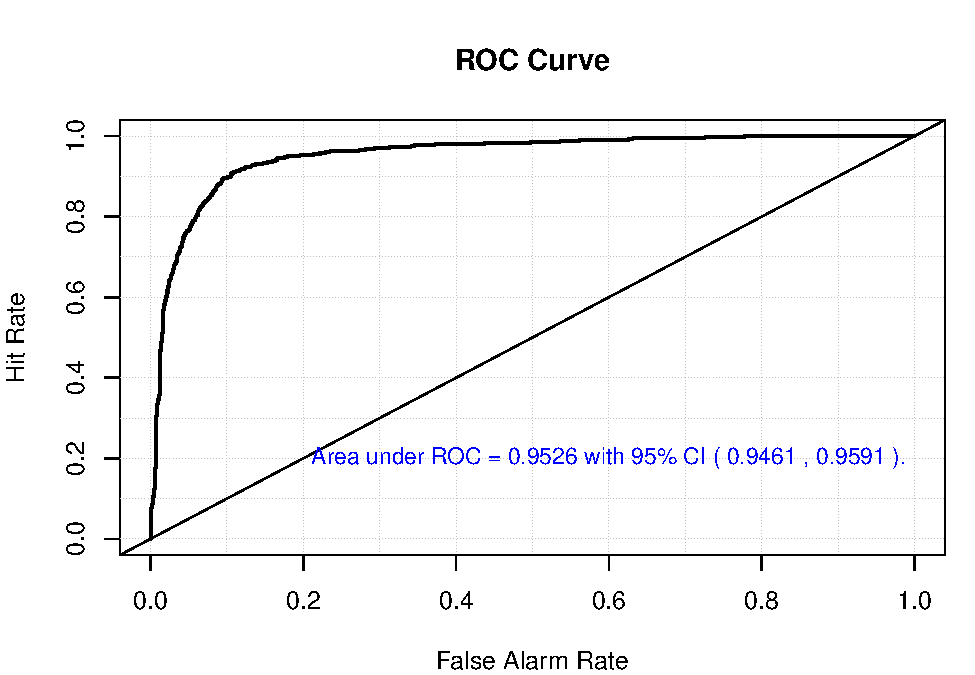
\includegraphics[width=0.9\linewidth]{OWUSU_project_files/figure-latex/unnamed-chunk-36-1}

\begin{Shaded}
\begin{Highlighting}[]
\NormalTok{auc.gam}\OtherTok{\textless{}{-}}\FunctionTok{round}\NormalTok{(gam.AUC}\SpecialCharTok{$}\NormalTok{cvAUC, }\AttributeTok{digits=}\DecValTok{4}\NormalTok{)}
\end{Highlighting}
\end{Shaded}

\hfill\break
\textbf{Comment:}

The AUC from the \textbf{GAM} model is 0.95 which is high and it tells
us that the model is a good fit and has good prediction accuracy.From
the output, it can be concluded from the confidence interval that the
model shows good discrimination.

\textbf{Plotting the (nonlinear) functional forms for continuous
predictors.}

\begin{Shaded}
\begin{Highlighting}[]
\FunctionTok{par}\NormalTok{(}\AttributeTok{mfrow=}\FunctionTok{c}\NormalTok{(}\DecValTok{3}\NormalTok{,}\DecValTok{3}\NormalTok{), }\AttributeTok{mar =} \FunctionTok{rep}\NormalTok{(}\DecValTok{4}\NormalTok{,}\DecValTok{4}\NormalTok{))}
\FunctionTok{plot}\NormalTok{(gam.fit2, }\AttributeTok{se =}\ConstantTok{TRUE}\NormalTok{)}
\end{Highlighting}
\end{Shaded}

\includegraphics[width=0.9\linewidth]{OWUSU_project_files/figure-latex/unnamed-chunk-37-1}

\textbf{Comment:}

In the backfitting algorithm, each smoothing parameter was calculated
adaptively. Because smoothing splines are utilized in this scenario, the
tuning parameter is automatically optimized using minimal GCV. Stepwise
selection with BIC was also used to choose variables. The considerable
nonlinearity displayed in the plots above demonstrates that the logistic
regression model is inadequate.

\newpage

\section{QUESTION 7 - Multivariate Adaptive Regression Splines (MARS)}

\begin{Shaded}
\begin{Highlighting}[]
\CommentTok{\# install.packages("earth")}
\FunctionTok{library}\NormalTok{(earth)    }\CommentTok{\# for MARS}
\FunctionTok{library}\NormalTok{(pdp)      }\CommentTok{\# for partial dependence plots}
\FunctionTok{library}\NormalTok{(vip)  }
\FunctionTok{library}\NormalTok{(caret)}\CommentTok{\# for variable importance plots}
\end{Highlighting}
\end{Shaded}

\subsection{Fitting MARS model}

\begin{Shaded}
\begin{Highlighting}[]
\NormalTok{fit.mars }\OtherTok{\textless{}{-}} \FunctionTok{earth}\NormalTok{(left }\SpecialCharTok{\textasciitilde{}}\NormalTok{ .,  }\AttributeTok{data =}\NormalTok{ D1, }\AttributeTok{degree=}\DecValTok{3}\NormalTok{, }\AttributeTok{ncross=}\DecValTok{3}\NormalTok{,}
    \AttributeTok{glm=}\FunctionTok{list}\NormalTok{(}\AttributeTok{family=}\FunctionTok{binomial}\NormalTok{(}\AttributeTok{link =} \StringTok{"logit"}\NormalTok{)), }
    \AttributeTok{pmethod=}\StringTok{"cv"}\NormalTok{, }\AttributeTok{nfold=}\DecValTok{10}\NormalTok{) }\CommentTok{\# tuning parameter degree = 3}

\FunctionTok{summary}\NormalTok{(fit.mars)}
\end{Highlighting}
\end{Shaded}

\begin{verbatim}
## Call: earth(formula=left~., data=D1, pmethod="cv",
##             glm=list(family=binomial(link="logit")), degree=3, nfold=10,
##             ncross=3)
## 
## GLM coefficients
##                                                                                           left
## (Intercept)                                                                            -4.3889
## h(0.15-satisfaction_level)                                                            152.8452
## h(satisfaction_level-0.15)                                                              4.3650
## h(3-number_project)                                                                    10.2973
## h(number_project-3)                                                                     0.8549
## h(satisfaction_level-0.15) * h(last_evaluation-0.99)                                  232.4778
## h(satisfaction_level-0.15) * h(0.99-last_evaluation)                                    2.0527
## h(0.23-satisfaction_level) * h(number_project-3)                                       -3.3099
## h(satisfaction_level-0.23) * h(number_project-3)                                       -0.6362
## h(0.38-satisfaction_level) * h(3-number_project)                                      -34.1717
## h(satisfaction_level-0.38) * h(3-number_project)                                      -21.4896
## h(satisfaction_level-0.15) * h(average_montly_hours-286)                                5.1564
## h(satisfaction_level-0.15) * h(286-average_montly_hours)                               -0.0425
## h(satisfaction_level-0.15) * h(time_spend_company-5)                                  -11.8019
## h(satisfaction_level-0.15) * h(5-time_spend_company)                                   -2.2165
## h(satisfaction_level-0.15) * h(time_spend_company-4)                                    8.4583
## h(0.46-last_evaluation) * h(3-number_project)                                        -135.4747
## h(last_evaluation-0.46) * h(3-number_project)                                         -16.8712
## h(3-number_project) * h(average_montly_hours-131)                                      -0.0223
## h(3-number_project) * h(131-average_montly_hours)                                      -0.3664
## h(3-number_project) * h(time_spend_company-3)                                          -1.2582
## h(3-number_project) * h(3-time_spend_company)                                          -3.5028
## h(number_project-3) * h(time_spend_company-5)                                          -0.5235
## h(number_project-3) * h(5-time_spend_company)                                           0.0546
## h(satisfaction_level-0.38) * h(last_evaluation-0.45) * h(3-number_project)             51.8794
## h(satisfaction_level-0.38) * h(0.45-last_evaluation) * h(3-number_project)         -11529.3660
## h(satisfaction_level-0.15) * h(0.99-last_evaluation) * h(time_spend_company-5)         20.0467
## h(satisfaction_level-0.15) * h(0.99-last_evaluation) * h(5-time_spend_company)         -1.4815
## h(satisfaction_level-0.15) * h(0.99-last_evaluation) * h(time_spend_company-4)        -18.7074
## h(satisfaction_level-0.23) * h(number_project-3) * h(time_spend_company-5)              1.7461
## h(satisfaction_level-0.23) * h(number_project-3) * h(5-time_spend_company)             -0.0998
## h(satisfaction_level-0.23) * h(number_project-3) * h(time_spend_company-4)             -0.2850
## h(satisfaction_level-0.15) * h(average_montly_hours-283) * h(5-time_spend_company)     -0.3454
## h(satisfaction_level-0.15) * h(283-average_montly_hours) * h(5-time_spend_company)      0.0174
## 
## GLM (family binomial, link logit):
##  nulldev   df       dev   df   devratio     AIC iters converged
##  10918.6 9998   2316.59 9965      0.788    2385    20         1
## 
## Earth selected 34 of 34 terms, and 5 of 18 predictors (pmethod="cv")
## Termination condition: Reached nk 37
## Importance: satisfaction_level, number_project, time_spend_company, ...
## Number of terms at each degree of interaction: 1 4 19 10
## Earth GRSq 0.7983041  RSq 0.8016191  mean.oof.RSq 0.7877309 (sd 0.0207)
## 
## pmethod="backward" would have selected:
##     30 terms 5 preds,  GRSq 0.7986453  RSq 0.801555  mean.oof.RSq 0.7852753
\end{verbatim}

\textbf{Model selection}

\begin{Shaded}
\begin{Highlighting}[]
\CommentTok{\# MODEL SELECTION}
\FunctionTok{par}\NormalTok{(}\AttributeTok{mfrow=}\FunctionTok{c}\NormalTok{(}\DecValTok{1}\NormalTok{, }\DecValTok{2}\NormalTok{), }\AttributeTok{mar=}\FunctionTok{rep}\NormalTok{(}\DecValTok{4}\NormalTok{,}\DecValTok{4}\NormalTok{))}
\NormalTok{q1 }\OtherTok{\textless{}{-}} \FunctionTok{plot}\NormalTok{(fit.mars, }\AttributeTok{which =} \DecValTok{1}\NormalTok{, }\AttributeTok{col.mean.infold.rsq=}\StringTok{"blue"}\NormalTok{, }
           \AttributeTok{col.infold.rsq=}\StringTok{"lightblue"}\NormalTok{,}\AttributeTok{col.grsq=}\DecValTok{0}\NormalTok{, }\AttributeTok{col.rsq=}\DecValTok{0}\NormalTok{, }
           \AttributeTok{col.vline=}\DecValTok{0}\NormalTok{, }\AttributeTok{col.oof.vline=}\DecValTok{0}\NormalTok{)}
\FunctionTok{plotres}\NormalTok{(fit.mars, }\AttributeTok{which=}\DecValTok{1}\NormalTok{, }\AttributeTok{info =} \ConstantTok{TRUE}\NormalTok{)}
\end{Highlighting}
\end{Shaded}

\includegraphics[width=0.9\linewidth]{OWUSU_project_files/figure-latex/unnamed-chunk-40-1}\\
\textbf{Comment:}

The plot on the left indicates training and testing performance (Rsq on
Y axis) obtained from the 10 fold cross validation performed thrice. The
performance on training data (blue curve) increases as we increase model
complexity; on independent data the performance (pink curve) increases
as well.

The plot on the right shows the best model selection (33 of 34 terms, 5
of 18 predictors using \textbf{pmethod=``cv''}) using green line,
indicating optimal terms as 33.

\hfill\break

\textbf{Variable importance plot}

\begin{Shaded}
\begin{Highlighting}[]
\FunctionTok{vip}\NormalTok{(fit.mars, }\AttributeTok{num\_features =} \DecValTok{10}\NormalTok{, }\AttributeTok{aesthetics =} \FunctionTok{list}\NormalTok{(}\AttributeTok{color =} \StringTok{"darkblue"}\NormalTok{, }\AttributeTok{fill =} \StringTok{"darkblue"}\NormalTok{)) }\SpecialCharTok{+} \FunctionTok{ggtitle}\NormalTok{(}\StringTok{"GCV"}\NormalTok{)}
\end{Highlighting}
\end{Shaded}

\includegraphics[width=0.9\linewidth]{OWUSU_project_files/figure-latex/unnamed-chunk-41-1}\\
\textbf{Comment:}

Fromt the \textbf{vip}, we see that \textbf{satisfaction\_level,
number\_project, time\_spend\_company} and \textbf{last\_evaluation} are
the four most influential variables; however, variable importance does
not tell us how our model is treating the non-linear patterns for each
feature. Also, if we look at the interaction terms our model retained,
we see interactions between different hinge functions.

\hfill\break
\textbf{Partial dependence plot}

\begin{Shaded}
\begin{Highlighting}[]
\CommentTok{\#par(mfrow=c(2,2), mar = rep(4,4))}
\NormalTok{q1 }\OtherTok{\textless{}{-}} \FunctionTok{partial}\NormalTok{(fit.mars, }\AttributeTok{pred.var =} \StringTok{"satisfaction\_level"}\NormalTok{, }\AttributeTok{grid.resolution =} \DecValTok{10}\NormalTok{)}\SpecialCharTok{\%\textgreater{}\%}\FunctionTok{autoplot}\NormalTok{()}
\NormalTok{q2 }\OtherTok{\textless{}{-}} \FunctionTok{partial}\NormalTok{(fit.mars, }\AttributeTok{pred.var =} \StringTok{"number\_project"}\NormalTok{, }\AttributeTok{grid.resolution =} \DecValTok{10}\NormalTok{)}\SpecialCharTok{\%\textgreater{}\%}\FunctionTok{autoplot}\NormalTok{()}
\NormalTok{q3 }\OtherTok{\textless{}{-}} \FunctionTok{partial}\NormalTok{(fit.mars, }\AttributeTok{pred.var =} \StringTok{"time\_spend\_company"}\NormalTok{, }\AttributeTok{grid.resolution =} \DecValTok{10}\NormalTok{)}\SpecialCharTok{\%\textgreater{}\%}\FunctionTok{autoplot}\NormalTok{()}
\NormalTok{q4 }\OtherTok{\textless{}{-}} \FunctionTok{partial}\NormalTok{(fit.mars, }\AttributeTok{pred.var =} \StringTok{"last\_evaluation"}\NormalTok{, }\AttributeTok{grid.resolution =} \DecValTok{10}\NormalTok{)}\SpecialCharTok{\%\textgreater{}\%}\FunctionTok{autoplot}\NormalTok{()}
\NormalTok{q5 }\OtherTok{\textless{}{-}} \FunctionTok{partial}\NormalTok{(fit.mars, }\AttributeTok{pred.var =} \FunctionTok{c}\NormalTok{(}\StringTok{"last\_evaluation"}\NormalTok{,}\StringTok{"satisfaction\_level"}\NormalTok{), }
              \AttributeTok{grid.resolution =} \DecValTok{10}\NormalTok{)}\SpecialCharTok{\%\textgreater{}\%}\FunctionTok{autoplot}\NormalTok{()}
\NormalTok{q6 }\OtherTok{\textless{}{-}} \FunctionTok{partial}\NormalTok{(fit.mars, }\AttributeTok{pred.var =} \FunctionTok{c}\NormalTok{(}\StringTok{"number\_project"}\NormalTok{,}\StringTok{"satisfaction\_level"}\NormalTok{), }
              \AttributeTok{grid.resolution =} \DecValTok{10}\NormalTok{)}\SpecialCharTok{\%\textgreater{}\%}\FunctionTok{autoplot}\NormalTok{()}

\FunctionTok{grid.arrange}\NormalTok{(q1,q2,q3,q4,q5,q6, }\AttributeTok{ncol =} \DecValTok{3}\NormalTok{)}
\end{Highlighting}
\end{Shaded}

\includegraphics[width=0.9\linewidth]{OWUSU_project_files/figure-latex/unnamed-chunk-42-1}\\
\textbf{Comment:}

From the first plot on the upper panel, we see that the is a sharp
increase in odds of an employee quit until a certain threshold of
satisfaction level, the odds start decreasing as satisfaction level
increases. Also, the variables \textbf{number\_project and
log(odds(left))} seems to be a directly proportional.

This 2-D plot gives us an idea about how the association of two
variables at a time on \textbf{log(odds(left))}. On the X- Axis we have
\textbf{satisfaction\_level} and on the Y-Axis we have
\textbf{last\_evaluation}. The variation is \textbf{log(odds(left))} is
indicated with the help of color scale (yellow indicating high odds and
dark violet indicating low odds).\\

\begin{Shaded}
\begin{Highlighting}[]
\NormalTok{yhat.mars }\OtherTok{\textless{}{-}} \FunctionTok{predict}\NormalTok{(fit.mars, }\AttributeTok{newdata=}\NormalTok{D2, }\AttributeTok{type=}\StringTok{"response"}\NormalTok{)}
\NormalTok{AUC.MARS }\OtherTok{\textless{}{-}} \FunctionTok{ci.cvAUC}\NormalTok{(}\AttributeTok{predictions=}\FunctionTok{as.vector}\NormalTok{(yhat.mars), }\AttributeTok{labels=}\NormalTok{yobs, }\AttributeTok{folds=}\DecValTok{1}\SpecialCharTok{:}\FunctionTok{length}\NormalTok{(yhat.mars), }\AttributeTok{confidence=}\FloatTok{0.95}\NormalTok{); AUC.MARS }
\end{Highlighting}
\end{Shaded}

\begin{verbatim}
## $cvAUC
## [1] 0.984323
## 
## $se
## [1] 0.002308812
## 
## $ci
## [1] 0.9797978 0.9888482
## 
## $confidence
## [1] 0.95
\end{verbatim}

\begin{Shaded}
\begin{Highlighting}[]
\NormalTok{auc.ci }\OtherTok{\textless{}{-}} \FunctionTok{round}\NormalTok{(AUC.MARS}\SpecialCharTok{$}\NormalTok{ci, }\AttributeTok{digits=}\DecValTok{4}\NormalTok{)}

\FunctionTok{library}\NormalTok{(verification)}
\NormalTok{mod.mars }\OtherTok{\textless{}{-}} \FunctionTok{verify}\NormalTok{(}\AttributeTok{obs=}\NormalTok{yobs, }\AttributeTok{pred=}\NormalTok{yhat.mars)}
\end{Highlighting}
\end{Shaded}

\begin{verbatim}
## If baseline is not included, baseline values  will be calculated from the  sample obs.
\end{verbatim}

\begin{Shaded}
\begin{Highlighting}[]
\FunctionTok{roc.plot}\NormalTok{(mod.mars, }\AttributeTok{plot.thres =} \ConstantTok{NULL}\NormalTok{, }\AttributeTok{main=}\StringTok{"ROC Curve from MARS"}\NormalTok{)}
\end{Highlighting}
\end{Shaded}

\begin{verbatim}
## Warning in roc.plot.default(c(1, 1, 1, 1, 1, 1, 1, 1, 1, 1, 1, 1, 1, 1, : Large
## amount of unique predictions used as thresholds. Consider specifying
## thresholds.
\end{verbatim}

\begin{Shaded}
\begin{Highlighting}[]
\FunctionTok{text}\NormalTok{(}\AttributeTok{x=}\FloatTok{0.6}\NormalTok{, }\AttributeTok{y=}\FloatTok{0.2}\NormalTok{, }\FunctionTok{paste}\NormalTok{(}\StringTok{"Area under ROC ="}\NormalTok{, }\FunctionTok{round}\NormalTok{(AUC.MARS}\SpecialCharTok{$}\NormalTok{cvAUC, }\AttributeTok{digits=}\DecValTok{4}\NormalTok{),}
    \AttributeTok{sep=}\StringTok{" "}\NormalTok{), }\AttributeTok{col=}\StringTok{"magenta"}\NormalTok{, }\AttributeTok{cex=}\FloatTok{1.2}\NormalTok{)}
\end{Highlighting}
\end{Shaded}

\includegraphics[width=0.9\linewidth]{OWUSU_project_files/figure-latex/unnamed-chunk-43-1}\\
\textbf{Comment:}

The AUC from the MARS is 0.98 which is high and it tells us that the
model is a good fit and has good prediction accuracy.

\newpage
\section{Question 8 - Project Pursuit Regression}

\begin{Shaded}
\begin{Highlighting}[]
\CommentTok{\# FIT PPR MODELS }
\CommentTok{\# nterms = number of terms to include in the final model.}
\CommentTok{\# max.terms = maximum number of terms to choose from when building the model.}

\NormalTok{D1}\SpecialCharTok{$}\NormalTok{left }\OtherTok{\textless{}{-}} \FunctionTok{ifelse}\NormalTok{(D1}\SpecialCharTok{$}\NormalTok{left}\SpecialCharTok{==}\StringTok{"stayed"}\NormalTok{, }\DecValTok{0}\NormalTok{, }\DecValTok{1}\NormalTok{)}
\NormalTok{fit0.ppr }\OtherTok{\textless{}{-}} \FunctionTok{ppr}\NormalTok{(left }\SpecialCharTok{\textasciitilde{}}\NormalTok{ ., }\AttributeTok{data =}\NormalTok{ D1, }
    \AttributeTok{nterms =} \DecValTok{2}\NormalTok{, }\AttributeTok{max.terms =} \DecValTok{10}\NormalTok{, }
    \AttributeTok{sm.method =} \StringTok{"supsmu"}\NormalTok{, }\AttributeTok{bass=}\DecValTok{3}\NormalTok{, }\AttributeTok{spen=}\DecValTok{0}\NormalTok{)}
\FunctionTok{summary}\NormalTok{(fit0.ppr)}
\end{Highlighting}
\end{Shaded}

\begin{verbatim}
## Call:
## ppr(formula = left ~ ., data = D1, nterms = 2, max.terms = 10, 
##     sm.method = "supsmu", bass = 3, spen = 0)
## 
## Goodness of fit:
##  2 terms  3 terms  4 terms  5 terms  6 terms  7 terms  8 terms  9 terms 
## 451.1104 450.2731 423.4635 467.2904 436.1631 438.1591   0.0000   0.0000 
## 10 terms 
##   0.0000 
## 
## Projection direction vectors ('alpha'):
##                       term 1        term 2       
## satisfaction_level     0.0012110979  0.0629132411
## last_evaluation       -0.0672644688  0.3751051150
## number_project        -0.0186586682  0.0821277029
## average_montly_hours  -0.0002477212  0.0012572350
## time_spend_company    -0.0343755565  0.0801642535
## Work_accident          0.0023366510 -0.0126586556
## promotion_last_5years  0.0070076745 -0.0366993631
## departmentaccounting   0.3144994785 -0.2894724412
## departmenthr           0.3148302260 -0.2834694747
## departmentIT           0.3149965761 -0.2913515756
## departmentmanagement   0.3135734074 -0.2862039390
## departmentmarketing    0.3145167534 -0.2897002318
## departmentproduct_mng  0.3146254501 -0.2886926810
## departmentRandD        0.3185114448 -0.2992944758
## departmentsales        0.3151921676 -0.2926202789
## departmentsupport      0.3164398008 -0.2900974043
## departmenttechnical    0.3153881345 -0.2882338908
## salary.L              -0.0009592769  0.0003331341
## salary.Q              -0.0003236076  0.0012576295
## 
## Coefficients of ridge terms ('beta'):
##    term 1    term 2 
## 0.2848580 0.4617535
\end{verbatim}

\begin{Shaded}
\begin{Highlighting}[]
\FunctionTok{par}\NormalTok{(}\AttributeTok{mfrow=}\FunctionTok{c}\NormalTok{(}\DecValTok{1}\NormalTok{,}\DecValTok{2}\NormalTok{), }\AttributeTok{mar=}\FunctionTok{rep}\NormalTok{(}\DecValTok{3}\NormalTok{,}\DecValTok{4}\NormalTok{))}
\FunctionTok{plot}\NormalTok{(fit0.ppr)}
\end{Highlighting}
\end{Shaded}

\includegraphics[width=0.9\linewidth]{OWUSU_project_files/figure-latex/unnamed-chunk-45-1}

\begin{Shaded}
\begin{Highlighting}[]
\NormalTok{yhat1.pp }\OtherTok{\textless{}{-}} \FunctionTok{predict}\NormalTok{(fit0.ppr, }\AttributeTok{newdata =}\NormalTok{ D2)}

\FunctionTok{qplot}\NormalTok{(yhat1.pp, }\AttributeTok{geom=}\StringTok{"histogram"}\NormalTok{, }\AttributeTok{xlab=}\StringTok{"Predicted"}\NormalTok{, }
      \AttributeTok{fill=}\FunctionTok{I}\NormalTok{(}\StringTok{"sky blue"}\NormalTok{), }\AttributeTok{col=}\FunctionTok{I}\NormalTok{(}\StringTok{"red"}\NormalTok{), }\AttributeTok{binwidth=}\FloatTok{0.05}\NormalTok{)}
\end{Highlighting}
\end{Shaded}

\begin{verbatim}
## Warning: `qplot()` was deprecated in ggplot2 3.4.0.
## This warning is displayed once every 8 hours.
## Call `lifecycle::last_lifecycle_warnings()` to see where this warning was
## generated.
\end{verbatim}

\includegraphics[width=0.9\linewidth]{OWUSU_project_files/figure-latex/unnamed-chunk-46-1}

\begin{Shaded}
\begin{Highlighting}[]
\CommentTok{\# SCALE PREDICTED Y INTO [0,1]}
\NormalTok{phat1.pp }\OtherTok{\textless{}{-}} \FunctionTok{as.vector}\NormalTok{(}\FunctionTok{scale}\NormalTok{(yhat1.pp, }\AttributeTok{center=}\FunctionTok{min}\NormalTok{(yhat1.pp), }
                   \AttributeTok{scale =} \FunctionTok{diff}\NormalTok{(}\FunctionTok{range}\NormalTok{(yhat1.pp))))}
\end{Highlighting}
\end{Shaded}

\begin{Shaded}
\begin{Highlighting}[]
\NormalTok{ppr.AUC }\OtherTok{\textless{}{-}} \FunctionTok{ci.cvAUC}\NormalTok{(}\AttributeTok{predictions=}\NormalTok{phat1.pp, }\AttributeTok{labels=}\NormalTok{yobs, }
                    \AttributeTok{folds=}\DecValTok{1}\SpecialCharTok{:}\FunctionTok{length}\NormalTok{(phat1.pp), }\AttributeTok{confidence=}\FloatTok{0.95}\NormalTok{)}
\NormalTok{ppr.auc.ci }\OtherTok{\textless{}{-}} \FunctionTok{round}\NormalTok{(ppr.AUC}\SpecialCharTok{$}\NormalTok{ci, }\AttributeTok{digits =} \DecValTok{4}\NormalTok{)}

\FunctionTok{library}\NormalTok{(verification)}
\NormalTok{mod.ppr }\OtherTok{\textless{}{-}} \FunctionTok{verify}\NormalTok{(}\AttributeTok{obs =}\NormalTok{ yobs, }\AttributeTok{pred =}\NormalTok{ phat1.pp)}
\end{Highlighting}
\end{Shaded}

\begin{verbatim}
## If baseline is not included, baseline values  will be calculated from the  sample obs.
\end{verbatim}

\begin{Shaded}
\begin{Highlighting}[]
\FunctionTok{roc.plot}\NormalTok{(mod.ppr, }\AttributeTok{plot.thres=}\ConstantTok{NULL}\NormalTok{)}
\end{Highlighting}
\end{Shaded}

\begin{verbatim}
## Warning in roc.plot.default(c(1, 1, 1, 1, 1, 1, 1, 1, 1, 1, 1, 1, 1, 1, : Large
## amount of unique predictions used as thresholds. Consider specifying
## thresholds.
\end{verbatim}

\begin{Shaded}
\begin{Highlighting}[]
\FunctionTok{text}\NormalTok{(}\AttributeTok{x=}\FloatTok{0.6}\NormalTok{, }\AttributeTok{y=}\FloatTok{0.2}\NormalTok{, }\FunctionTok{paste}\NormalTok{(}\StringTok{"Area under ROC = "}\NormalTok{, }
                         \FunctionTok{round}\NormalTok{(ppr.AUC}\SpecialCharTok{$}\NormalTok{cvAUC, }\AttributeTok{digits =} \DecValTok{4}\NormalTok{), }
                         \StringTok{"with 95\% CI ("}\NormalTok{,}
\NormalTok{                         ppr.auc.ci[}\DecValTok{1}\NormalTok{], }\StringTok{","}\NormalTok{, ppr.auc.ci[}\DecValTok{2}\NormalTok{], }
                         \StringTok{")."}\NormalTok{, }\AttributeTok{sep =} \StringTok{" "}\NormalTok{), }\AttributeTok{col=}\StringTok{"blue"}\NormalTok{, }\AttributeTok{cex =}\FloatTok{1.2}\NormalTok{)}
\end{Highlighting}
\end{Shaded}

\includegraphics[width=0.9\linewidth]{OWUSU_project_files/figure-latex/unnamed-chunk-48-1}\\
The AUC from the PPR is 0.97 which is high and it tells us that the
model is a good fit and has good prediction accuracy.

\hfill\break

\section{Model Comparison}

\begin{Shaded}
\begin{Highlighting}[]
\FunctionTok{library}\NormalTok{(kableExtra)}
\NormalTok{Measure }\OtherTok{\textless{}{-}} \FunctionTok{c}\NormalTok{(AUC.LASSO}\SpecialCharTok{$}\NormalTok{cvAUC, AUC.RF}\SpecialCharTok{$}\NormalTok{cvAUC, gam.AUC}\SpecialCharTok{$}\NormalTok{cvAUC, AUC.MARS}\SpecialCharTok{$}\NormalTok{cvAUC,}
\NormalTok{             ppr.AUC}\SpecialCharTok{$}\NormalTok{cvAUC)}
\NormalTok{mod }\OtherTok{\textless{}{-}} \FunctionTok{data.frame}\NormalTok{(}\StringTok{"Method"}\OtherTok{=} \FunctionTok{c}\NormalTok{(}\StringTok{"LASSO"}\NormalTok{,}\StringTok{"Random Forest"}\NormalTok{,}\StringTok{"GAM"}\NormalTok{,}\StringTok{"MARS"}\NormalTok{,}\StringTok{"PPR"}\NormalTok{),}
                       \StringTok{"AUC"}\OtherTok{=}\NormalTok{ Measure)}

\NormalTok{knitr}\SpecialCharTok{::}\FunctionTok{kable}\NormalTok{(mod, }\AttributeTok{booktabs =}\NormalTok{ T, }\AttributeTok{format =} \StringTok{"markdown"}\NormalTok{, }\AttributeTok{digits =} \DecValTok{3}\NormalTok{) }\SpecialCharTok{\%\textgreater{}\%}
  \FunctionTok{kable\_paper}\NormalTok{(}\StringTok{"hover"}\NormalTok{, }\AttributeTok{full\_width =}\NormalTok{ F)}\SpecialCharTok{\%\textgreater{}\%} 
  \FunctionTok{kable\_styling}\NormalTok{(}\AttributeTok{font\_size =} \DecValTok{12}\NormalTok{,}\AttributeTok{bootstrap\_options =} \StringTok{"striped"}\NormalTok{,}
                     \AttributeTok{full\_width =}\NormalTok{ F, }\AttributeTok{latex\_options =} \FunctionTok{c}\NormalTok{(}\StringTok{"HOLD\_position"}\NormalTok{))}
\end{Highlighting}
\end{Shaded}

\begin{longtable}[]{@{}lr@{}}
\toprule\noalign{}
Method & AUC \\
\midrule\noalign{}
\endhead
\bottomrule\noalign{}
\endlastfoot
LASSO & 0.811 \\
Random Forest & 0.992 \\
GAM & 0.953 \\
MARS & 0.984 \\
PPR & 0.965 \\
\end{longtable}

\textbf{Comment:}

From the output above, we can conclude that among all the five
supervised learning approaches used, the \textbf{Random Forest} gives
favorable result since its model produced relatively high area under the
receiver operating characteristic curve, that is \(AUC=\) 0.99.

\end{document}
